\documentclass[twoside]{book}

% Packages required by doxygen
\usepackage{fixltx2e}
\usepackage{calc}
\usepackage{doxygen}
\usepackage[export]{adjustbox} % also loads graphicx
\usepackage{graphicx}
\usepackage[utf8]{inputenc}
\usepackage{makeidx}
\usepackage{multicol}
\usepackage{multirow}
\PassOptionsToPackage{warn}{textcomp}
\usepackage{textcomp}
\usepackage[nointegrals]{wasysym}
\usepackage[table]{xcolor}

% Font selection
\usepackage[T1]{fontenc}
\usepackage[scaled=.90]{helvet}
\usepackage{courier}
\usepackage{amssymb}
\usepackage{sectsty}
\renewcommand{\familydefault}{\sfdefault}
\allsectionsfont{%
  \fontseries{bc}\selectfont%
  \color{darkgray}%
}
\renewcommand{\DoxyLabelFont}{%
  \fontseries{bc}\selectfont%
  \color{darkgray}%
}
\newcommand{\+}{\discretionary{\mbox{\scriptsize$\hookleftarrow$}}{}{}}

% Page & text layout
\usepackage{geometry}
\geometry{%
  a4paper,%
  top=2.5cm,%
  bottom=2.5cm,%
  left=2.5cm,%
  right=2.5cm%
}
\tolerance=750
\hfuzz=15pt
\hbadness=750
\setlength{\emergencystretch}{15pt}
\setlength{\parindent}{0cm}
\setlength{\parskip}{3ex plus 2ex minus 2ex}
\makeatletter
\renewcommand{\paragraph}{%
  \@startsection{paragraph}{4}{0ex}{-1.0ex}{1.0ex}{%
    \normalfont\normalsize\bfseries\SS@parafont%
  }%
}
\renewcommand{\subparagraph}{%
  \@startsection{subparagraph}{5}{0ex}{-1.0ex}{1.0ex}{%
    \normalfont\normalsize\bfseries\SS@subparafont%
  }%
}
\makeatother

% Headers & footers
\usepackage{fancyhdr}
\pagestyle{fancyplain}
\fancyhead[LE]{\fancyplain{}{\bfseries\thepage}}
\fancyhead[CE]{\fancyplain{}{}}
\fancyhead[RE]{\fancyplain{}{\bfseries\leftmark}}
\fancyhead[LO]{\fancyplain{}{\bfseries\rightmark}}
\fancyhead[CO]{\fancyplain{}{}}
\fancyhead[RO]{\fancyplain{}{\bfseries\thepage}}
\fancyfoot[LE]{\fancyplain{}{}}
\fancyfoot[CE]{\fancyplain{}{}}
\fancyfoot[RE]{\fancyplain{}{\bfseries\scriptsize Generated by Doxygen }}
\fancyfoot[LO]{\fancyplain{}{\bfseries\scriptsize Generated by Doxygen }}
\fancyfoot[CO]{\fancyplain{}{}}
\fancyfoot[RO]{\fancyplain{}{}}
\renewcommand{\footrulewidth}{0.4pt}
\renewcommand{\chaptermark}[1]{%
  \markboth{#1}{}%
}
\renewcommand{\sectionmark}[1]{%
  \markright{\thesection\ #1}%
}

% Indices & bibliography
\usepackage{natbib}
\usepackage[titles]{tocloft}
\setcounter{tocdepth}{3}
\setcounter{secnumdepth}{5}
\makeindex

% Hyperlinks (required, but should be loaded last)
\usepackage{ifpdf}
\ifpdf
  \usepackage[pdftex,pagebackref=true]{hyperref}
\else
  \usepackage[ps2pdf,pagebackref=true]{hyperref}
\fi
\hypersetup{%
  colorlinks=true,%
  linkcolor=blue,%
  citecolor=blue,%
  unicode%
}

% Custom commands
\newcommand{\clearemptydoublepage}{%
  \newpage{\pagestyle{empty}\cleardoublepage}%
}

\usepackage{caption}
\captionsetup{labelsep=space,justification=centering,font={bf},singlelinecheck=off,skip=4pt,position=top}

%===== C O N T E N T S =====

\begin{document}

% Titlepage & ToC
\hypersetup{pageanchor=false,
             bookmarksnumbered=true,
             pdfencoding=unicode
            }
\pagenumbering{alph}
\begin{titlepage}
\vspace*{7cm}
\begin{center}%
{\Large Music\+Light }\\
\vspace*{1cm}
{\large Generated by Doxygen 1.8.13}\\
\end{center}
\end{titlepage}
\clearemptydoublepage
\pagenumbering{roman}
\tableofcontents
\clearemptydoublepage
\pagenumbering{arabic}
\hypersetup{pageanchor=true}

%--- Begin generated contents ---
\chapter{Hierarchical Index}
\section{Class Hierarchy}
This inheritance list is sorted roughly, but not completely, alphabetically\+:\begin{DoxyCompactList}
\item \contentsline{section}{light\+Music\+:\+:buzzer}{\pageref{classlight_music_1_1buzzer}}{}
\item \contentsline{section}{light\+Music\+:\+:key\+Matrix}{\pageref{classlight_music_1_1key_matrix}}{}
\begin{DoxyCompactList}
\item \contentsline{section}{light\+Music\+:\+:midi}{\pageref{classlight_music_1_1midi}}{}
\end{DoxyCompactList}
\item \contentsline{section}{light\+Music\+:\+:max7219}{\pageref{classlight_music_1_1max7219}}{}
\end{DoxyCompactList}

\chapter{Class Index}
\section{Class List}
Here are the classes, structs, unions and interfaces with brief descriptions\+:\begin{DoxyCompactList}
\item\contentsline{section}{\hyperlink{classlight_music_1_1buzzer}{light\+Music\+::buzzer} }{\pageref{classlight_music_1_1buzzer}}{}
\item\contentsline{section}{\hyperlink{classlight_music_1_1key_matrix}{light\+Music\+::key\+Matrix} \\*Class for a \hyperlink{classlight_music_1_1key_matrix}{key\+Matrix} }{\pageref{classlight_music_1_1key_matrix}}{}
\item\contentsline{section}{\hyperlink{classlight_music_1_1max7219}{light\+Music\+::max7219} \\*Class to set and draw on the \hyperlink{classlight_music_1_1max7219}{max7219} 8x8 matrixes }{\pageref{classlight_music_1_1max7219}}{}
\item\contentsline{section}{\hyperlink{classlight_music_1_1midi}{light\+Music\+::midi} \\*Class to send midi messages to tx pin }{\pageref{classlight_music_1_1midi}}{}
\end{DoxyCompactList}

\chapter{File Index}
\section{File List}
Here is a list of all documented files with brief descriptions\+:\begin{DoxyCompactList}
\item\contentsline{section}{C\+:/ti-\/software/lightmusic/lightmusic/{\bfseries buzzer.\+hpp} }{\pageref{buzzer_8hpp}}{}
\item\contentsline{section}{C\+:/ti-\/software/lightmusic/lightmusic/\hyperlink{constants8x8chars_8hpp}{constants8x8chars.\+hpp} }{\pageref{constants8x8chars_8hpp}}{}
\item\contentsline{section}{C\+:/ti-\/software/lightmusic/lightmusic/\hyperlink{constantsmax7219_8hpp}{constantsmax7219.\+hpp} }{\pageref{constantsmax7219_8hpp}}{}
\item\contentsline{section}{C\+:/ti-\/software/lightmusic/lightmusic/\hyperlink{constantsmidi_8hpp}{constantsmidi.\+hpp} }{\pageref{constantsmidi_8hpp}}{}
\item\contentsline{section}{C\+:/ti-\/software/lightmusic/lightmusic/{\bfseries keymatrix.\+hpp} }{\pageref{keymatrix_8hpp}}{}
\item\contentsline{section}{C\+:/ti-\/software/lightmusic/lightmusic/{\bfseries lightmusiclib.\+hpp} }{\pageref{lightmusiclib_8hpp}}{}
\item\contentsline{section}{C\+:/ti-\/software/lightmusic/lightmusic/{\bfseries max7219.\+hpp} }{\pageref{max7219_8hpp}}{}
\item\contentsline{section}{C\+:/ti-\/software/lightmusic/lightmusic/{\bfseries midi.\+hpp} }{\pageref{midi_8hpp}}{}
\end{DoxyCompactList}

\chapter{Class Documentation}
\hypertarget{classlight_music_1_1buzzer}{}\section{light\+Music\+:\+:buzzer Class Reference}
\label{classlight_music_1_1buzzer}\index{light\+Music\+::buzzer@{light\+Music\+::buzzer}}
\subsection*{Public Member Functions}
\begin{DoxyCompactItemize}
\item 
\hyperlink{classlight_music_1_1buzzer_aa708682093bf3831c1d54e75ef21eb63}{buzzer} (hwlib\+::target\+::pin\+\_\+out sig)
\begin{DoxyCompactList}\small\item\em Constructor. \end{DoxyCompactList}\item 
void \hyperlink{classlight_music_1_1buzzer_a5fed541127d6e863a4981b79388ab1bb}{tone} (int hertz)
\begin{DoxyCompactList}\small\item\em play the tone by given hertz \end{DoxyCompactList}\item 
int \hyperlink{classlight_music_1_1buzzer_a51b71d6a57ac66340e67f641fb3d3a69}{key\+Midi\+Map\+To\+Hertz} (int Key\+Midi\+Number)
\begin{DoxyCompactList}\small\item\em calculate the hertz by given midi\+Key\+Number and returns the hertz in int \end{DoxyCompactList}\end{DoxyCompactItemize}


\subsection{Constructor \& Destructor Documentation}
\mbox{\Hypertarget{classlight_music_1_1buzzer_aa708682093bf3831c1d54e75ef21eb63}\label{classlight_music_1_1buzzer_aa708682093bf3831c1d54e75ef21eb63}} 
\index{light\+Music\+::buzzer@{light\+Music\+::buzzer}!buzzer@{buzzer}}
\index{buzzer@{buzzer}!light\+Music\+::buzzer@{light\+Music\+::buzzer}}
\subsubsection{\texorpdfstring{buzzer()}{buzzer()}}
{\footnotesize\ttfamily light\+Music\+::buzzer\+::buzzer (\begin{DoxyParamCaption}\item[{hwlib\+::target\+::pin\+\_\+out}]{sig }\end{DoxyParamCaption})}



Constructor. 


\begin{DoxyParams}{Parameters}
{\em sig} & signal output pin for the buzzer\\
\hline
\end{DoxyParams}
sets the output pin to the given output pin 

\subsection{Member Function Documentation}
\mbox{\Hypertarget{classlight_music_1_1buzzer_a51b71d6a57ac66340e67f641fb3d3a69}\label{classlight_music_1_1buzzer_a51b71d6a57ac66340e67f641fb3d3a69}} 
\index{light\+Music\+::buzzer@{light\+Music\+::buzzer}!key\+Midi\+Map\+To\+Hertz@{key\+Midi\+Map\+To\+Hertz}}
\index{key\+Midi\+Map\+To\+Hertz@{key\+Midi\+Map\+To\+Hertz}!light\+Music\+::buzzer@{light\+Music\+::buzzer}}
\subsubsection{\texorpdfstring{key\+Midi\+Map\+To\+Hertz()}{keyMidiMapToHertz()}}
{\footnotesize\ttfamily int light\+Music\+::buzzer\+::key\+Midi\+Map\+To\+Hertz (\begin{DoxyParamCaption}\item[{int}]{Key\+Midi\+Number }\end{DoxyParamCaption})}



calculate the hertz by given midi\+Key\+Number and returns the hertz in int 


\begin{DoxyParams}{Parameters}
{\em key\+Midi\+Number} & the number of the key \\
\hline
\end{DoxyParams}
\begin{DoxyReturn}{Returns}
returns hertz in int 
\end{DoxyReturn}
\mbox{\Hypertarget{classlight_music_1_1buzzer_a5fed541127d6e863a4981b79388ab1bb}\label{classlight_music_1_1buzzer_a5fed541127d6e863a4981b79388ab1bb}} 
\index{light\+Music\+::buzzer@{light\+Music\+::buzzer}!tone@{tone}}
\index{tone@{tone}!light\+Music\+::buzzer@{light\+Music\+::buzzer}}
\subsubsection{\texorpdfstring{tone()}{tone()}}
{\footnotesize\ttfamily void light\+Music\+::buzzer\+::tone (\begin{DoxyParamCaption}\item[{int}]{hertz }\end{DoxyParamCaption})}



play the tone by given hertz 


\begin{DoxyParams}{Parameters}
{\em hertz} & the hertz in ints \\
\hline
\end{DoxyParams}


The documentation for this class was generated from the following files\+:\begin{DoxyCompactItemize}
\item 
C\+:/ti-\/software/lightmusic/lightmusic/buzzer.\+hpp\item 
C\+:/ti-\/software/lightmusic/lightmusic/buzzer.\+cpp\end{DoxyCompactItemize}

\hypertarget{classlight_music_1_1key_matrix}{}\section{light\+Music\+:\+:key\+Matrix Class Reference}
\label{classlight_music_1_1key_matrix}\index{light\+Music\+::key\+Matrix@{light\+Music\+::key\+Matrix}}


Class for a \hyperlink{classlight_music_1_1key_matrix}{key\+Matrix}.  




{\ttfamily \#include $<$keymatrix.\+hpp$>$}

Inheritance diagram for light\+Music\+:\+:key\+Matrix\+:\begin{figure}[H]
\begin{center}
\leavevmode
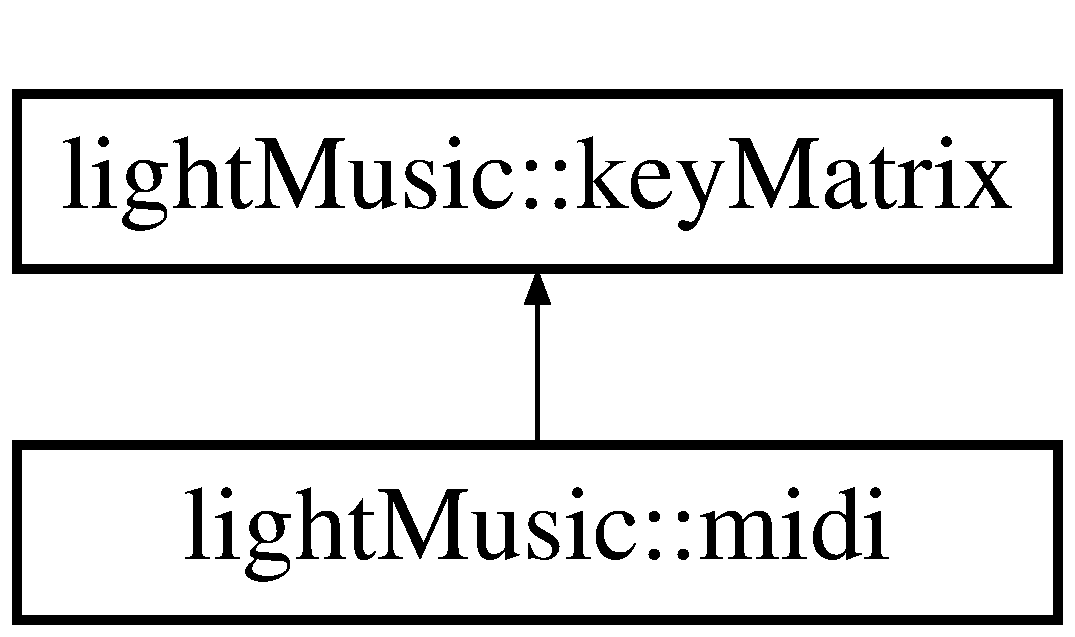
\includegraphics[height=2.000000cm]{classlight_music_1_1key_matrix}
\end{center}
\end{figure}
\subsection*{Public Member Functions}
\begin{DoxyCompactItemize}
\item 
\hyperlink{classlight_music_1_1key_matrix_a20157eac9f3c3c056101178beeae5cc2}{key\+Matrix} (hwlib\+::target\+::pin\+\_\+in \&row1, hwlib\+::target\+::pin\+\_\+in \&row2, hwlib\+::target\+::pin\+\_\+in \&row3, hwlib\+::target\+::pin\+\_\+in \&row4, const int \&\hyperlink{classlight_music_1_1key_matrix_ab9fa44924cb5e674870f2602f92b39d3}{num\+Cols})
\begin{DoxyCompactList}\small\item\em Constructor. \end{DoxyCompactList}\item 
void \hyperlink{classlight_music_1_1key_matrix_ab14732662e5383219d953562dca72093}{set} ()
\begin{DoxyCompactList}\small\item\em Sets every button of the matrix on false. \end{DoxyCompactList}\item 
void \hyperlink{classlight_music_1_1key_matrix_a12c6a2c68f752505b080b9ec5a43601b}{scan\+Column} (const int \hyperlink{classlight_music_1_1key_matrix_ab9fa44924cb5e674870f2602f92b39d3}{num\+Cols}, hwlib\+::target\+::pin\+\_\+out \&latch\+Pin, hwlib\+::target\+::pin\+\_\+out \&data\+Pin, hwlib\+::target\+::pin\+\_\+out \&clock\+Pin)
\begin{DoxyCompactList}\small\item\em Send to each column line a 1. \end{DoxyCompactList}\item 
bool $\ast$ \hyperlink{classlight_music_1_1key_matrix_a11147e2bed1cc44d6127d23f6d1750be}{get\+Row\+Value} ()
\begin{DoxyCompactList}\small\item\em give the value of the row in a array \end{DoxyCompactList}\item 
int \hyperlink{classlight_music_1_1key_matrix_ac57a81f084a6eed8aea1db203ddebcbe}{get\+Num\+Rows} ()
\begin{DoxyCompactList}\small\item\em give the number of rows back \end{DoxyCompactList}\item 
int \hyperlink{classlight_music_1_1key_matrix_a26d5321912cf6eb7e4cb653ae52f2127}{get\+Num\+Cols} ()
\begin{DoxyCompactList}\small\item\em give the number of cols back \end{DoxyCompactList}\item 
bool \hyperlink{classlight_music_1_1key_matrix_aa24325eefb6e1d1c658a95414d178152}{get\+Key\+Pressed} (int row\+Ctr, int col\+Ctr)
\begin{DoxyCompactList}\small\item\em get the value of a keypressed on a given location \end{DoxyCompactList}\item 
void \hyperlink{classlight_music_1_1key_matrix_a6b14156dc4fe97c317878e638e25b065}{set\+Key\+Pressed} (int rowctr, int colctr, bool data)
\begin{DoxyCompactList}\small\item\em set the given data to keypressed on a given location \end{DoxyCompactList}\item 
int \hyperlink{classlight_music_1_1key_matrix_a0da0736764140f22eeb6874f4b5d2080}{get\+Key\+To\+Midi\+Map} (int rowctr, int colctr)
\begin{DoxyCompactList}\small\item\em get the value of a keytomidimap on a given location \end{DoxyCompactList}\item 
uint8\+\_\+t \hyperlink{classlight_music_1_1key_matrix_a3e25f2258ac3be18fe6e85f6cf0cccfa}{get\+Key\+To\+Midi\+Map8t} (int rowctr, int colctr)
\begin{DoxyCompactList}\small\item\em get the value of a keytomidimap on a given location \end{DoxyCompactList}\item 
void \hyperlink{classlight_music_1_1key_matrix_a21cce0cc53842750aac7fad18652e697}{min\+Max\+Velocity} (int number, bool min\+Max)
\begin{DoxyCompactList}\small\item\em set the velocity by \char`\"{}min/max number + velocity\char`\"{} \end{DoxyCompactList}\item 
int \hyperlink{classlight_music_1_1key_matrix_ac0598a969eaf6469ccac2206f4456f3b}{get\+Velocity} ()
\begin{DoxyCompactList}\small\item\em get the velocity \end{DoxyCompactList}\item 
void \hyperlink{classlight_music_1_1key_matrix_a299fd57c69d7afa13da683b3e2e59368}{min\+Max\+Quant\+Of\+Pres\+Keys} (bool min\+Max)
\begin{DoxyCompactList}\small\item\em set 1 minus/plus the int quant\+Of\+Press\+Keys \end{DoxyCompactList}\item 
int \hyperlink{classlight_music_1_1key_matrix_a3508804c32287b9694bf2329aa4f9ece}{get\+Quant\+Of\+Pres\+Keys} ()
\begin{DoxyCompactList}\small\item\em get int quantofpreskeys \end{DoxyCompactList}\end{DoxyCompactItemize}
\subsection*{Protected Attributes}
\begin{DoxyCompactItemize}
\item 
\mbox{\Hypertarget{classlight_music_1_1key_matrix_afbad6c22d812070e3ad0fbeefe73b94b}\label{classlight_music_1_1key_matrix_afbad6c22d812070e3ad0fbeefe73b94b}} 
int \hyperlink{classlight_music_1_1key_matrix_afbad6c22d812070e3ad0fbeefe73b94b}{num\+Rows} = 4
\begin{DoxyCompactList}\small\item\em Number of all the rows. \end{DoxyCompactList}\item 
\mbox{\Hypertarget{classlight_music_1_1key_matrix_ab9fa44924cb5e674870f2602f92b39d3}\label{classlight_music_1_1key_matrix_ab9fa44924cb5e674870f2602f92b39d3}} 
int \hyperlink{classlight_music_1_1key_matrix_ab9fa44924cb5e674870f2602f92b39d3}{num\+Cols}
\begin{DoxyCompactList}\small\item\em Number of all the colums. \end{DoxyCompactList}\end{DoxyCompactItemize}


\subsection{Detailed Description}
Class for a \hyperlink{classlight_music_1_1key_matrix}{key\+Matrix}. 

\hyperlink{classlight_music_1_1key_matrix}{key\+Matrix} is a class with 5 functions, which makes it possible to setup the \hyperlink{classlight_music_1_1key_matrix}{key\+Matrix}, scan the colums by using the shiftout function. And to return the number of cols and rows 

\subsection{Constructor \& Destructor Documentation}
\mbox{\Hypertarget{classlight_music_1_1key_matrix_a20157eac9f3c3c056101178beeae5cc2}\label{classlight_music_1_1key_matrix_a20157eac9f3c3c056101178beeae5cc2}} 
\index{light\+Music\+::key\+Matrix@{light\+Music\+::key\+Matrix}!key\+Matrix@{key\+Matrix}}
\index{key\+Matrix@{key\+Matrix}!light\+Music\+::key\+Matrix@{light\+Music\+::key\+Matrix}}
\subsubsection{\texorpdfstring{key\+Matrix()}{keyMatrix()}}
{\footnotesize\ttfamily light\+Music\+::key\+Matrix\+::key\+Matrix (\begin{DoxyParamCaption}\item[{hwlib\+::target\+::pin\+\_\+in \&}]{row1,  }\item[{hwlib\+::target\+::pin\+\_\+in \&}]{row2,  }\item[{hwlib\+::target\+::pin\+\_\+in \&}]{row3,  }\item[{hwlib\+::target\+::pin\+\_\+in \&}]{row4,  }\item[{const int \&}]{num\+Cols }\end{DoxyParamCaption})}



Constructor. 


\begin{DoxyParams}{Parameters}
{\em row} & Port of al the row inputs \\
\hline
{\em num\+Cols} & Number of all the colums \\
\hline
{\em note} & Number of the first button\textquotesingle{}s key\\
\hline
\end{DoxyParams}
sets row with param row, num\+\_\+row with the number of the pins of row, num\+\_\+cols with param num\+\_\+cols 

\subsection{Member Function Documentation}
\mbox{\Hypertarget{classlight_music_1_1key_matrix_aa24325eefb6e1d1c658a95414d178152}\label{classlight_music_1_1key_matrix_aa24325eefb6e1d1c658a95414d178152}} 
\index{light\+Music\+::key\+Matrix@{light\+Music\+::key\+Matrix}!get\+Key\+Pressed@{get\+Key\+Pressed}}
\index{get\+Key\+Pressed@{get\+Key\+Pressed}!light\+Music\+::key\+Matrix@{light\+Music\+::key\+Matrix}}
\subsubsection{\texorpdfstring{get\+Key\+Pressed()}{getKeyPressed()}}
{\footnotesize\ttfamily bool light\+Music\+::key\+Matrix\+::get\+Key\+Pressed (\begin{DoxyParamCaption}\item[{int}]{row\+Ctr,  }\item[{int}]{col\+Ctr }\end{DoxyParamCaption})}



get the value of a keypressed on a given location 


\begin{DoxyParams}{Parameters}
{\em rowctr} & which row \\
\hline
{\em colctr} & which column \\
\hline
\end{DoxyParams}
\begin{DoxyReturn}{Returns}
bool of a the given location of the keypressed 
\end{DoxyReturn}
\mbox{\Hypertarget{classlight_music_1_1key_matrix_a0da0736764140f22eeb6874f4b5d2080}\label{classlight_music_1_1key_matrix_a0da0736764140f22eeb6874f4b5d2080}} 
\index{light\+Music\+::key\+Matrix@{light\+Music\+::key\+Matrix}!get\+Key\+To\+Midi\+Map@{get\+Key\+To\+Midi\+Map}}
\index{get\+Key\+To\+Midi\+Map@{get\+Key\+To\+Midi\+Map}!light\+Music\+::key\+Matrix@{light\+Music\+::key\+Matrix}}
\subsubsection{\texorpdfstring{get\+Key\+To\+Midi\+Map()}{getKeyToMidiMap()}}
{\footnotesize\ttfamily int light\+Music\+::key\+Matrix\+::get\+Key\+To\+Midi\+Map (\begin{DoxyParamCaption}\item[{int}]{rowctr,  }\item[{int}]{colctr }\end{DoxyParamCaption})}



get the value of a keytomidimap on a given location 


\begin{DoxyParams}{Parameters}
{\em rowctr} & which row \\
\hline
{\em colctr} & which column \\
\hline
\end{DoxyParams}
\begin{DoxyReturn}{Returns}
int of the key on the given location 
\end{DoxyReturn}
\mbox{\Hypertarget{classlight_music_1_1key_matrix_a3e25f2258ac3be18fe6e85f6cf0cccfa}\label{classlight_music_1_1key_matrix_a3e25f2258ac3be18fe6e85f6cf0cccfa}} 
\index{light\+Music\+::key\+Matrix@{light\+Music\+::key\+Matrix}!get\+Key\+To\+Midi\+Map8t@{get\+Key\+To\+Midi\+Map8t}}
\index{get\+Key\+To\+Midi\+Map8t@{get\+Key\+To\+Midi\+Map8t}!light\+Music\+::key\+Matrix@{light\+Music\+::key\+Matrix}}
\subsubsection{\texorpdfstring{get\+Key\+To\+Midi\+Map8t()}{getKeyToMidiMap8t()}}
{\footnotesize\ttfamily uint8\+\_\+t light\+Music\+::key\+Matrix\+::get\+Key\+To\+Midi\+Map8t (\begin{DoxyParamCaption}\item[{int}]{rowctr,  }\item[{int}]{colctr }\end{DoxyParamCaption})}



get the value of a keytomidimap on a given location 


\begin{DoxyParams}{Parameters}
{\em rowctr} & which row \\
\hline
{\em colctr} & which column \\
\hline
\end{DoxyParams}
\begin{DoxyReturn}{Returns}
uint8\+\_\+t of the key on the given location 
\end{DoxyReturn}
\mbox{\Hypertarget{classlight_music_1_1key_matrix_a26d5321912cf6eb7e4cb653ae52f2127}\label{classlight_music_1_1key_matrix_a26d5321912cf6eb7e4cb653ae52f2127}} 
\index{light\+Music\+::key\+Matrix@{light\+Music\+::key\+Matrix}!get\+Num\+Cols@{get\+Num\+Cols}}
\index{get\+Num\+Cols@{get\+Num\+Cols}!light\+Music\+::key\+Matrix@{light\+Music\+::key\+Matrix}}
\subsubsection{\texorpdfstring{get\+Num\+Cols()}{getNumCols()}}
{\footnotesize\ttfamily int light\+Music\+::key\+Matrix\+::get\+Num\+Cols (\begin{DoxyParamCaption}{ }\end{DoxyParamCaption})}



give the number of cols back 

\begin{DoxyReturn}{Returns}
int of cols in the keymatrix 
\end{DoxyReturn}
\mbox{\Hypertarget{classlight_music_1_1key_matrix_ac57a81f084a6eed8aea1db203ddebcbe}\label{classlight_music_1_1key_matrix_ac57a81f084a6eed8aea1db203ddebcbe}} 
\index{light\+Music\+::key\+Matrix@{light\+Music\+::key\+Matrix}!get\+Num\+Rows@{get\+Num\+Rows}}
\index{get\+Num\+Rows@{get\+Num\+Rows}!light\+Music\+::key\+Matrix@{light\+Music\+::key\+Matrix}}
\subsubsection{\texorpdfstring{get\+Num\+Rows()}{getNumRows()}}
{\footnotesize\ttfamily int light\+Music\+::key\+Matrix\+::get\+Num\+Rows (\begin{DoxyParamCaption}{ }\end{DoxyParamCaption})}



give the number of rows back 

\begin{DoxyReturn}{Returns}
number of rows in the keymatrix 
\end{DoxyReturn}
\mbox{\Hypertarget{classlight_music_1_1key_matrix_a3508804c32287b9694bf2329aa4f9ece}\label{classlight_music_1_1key_matrix_a3508804c32287b9694bf2329aa4f9ece}} 
\index{light\+Music\+::key\+Matrix@{light\+Music\+::key\+Matrix}!get\+Quant\+Of\+Pres\+Keys@{get\+Quant\+Of\+Pres\+Keys}}
\index{get\+Quant\+Of\+Pres\+Keys@{get\+Quant\+Of\+Pres\+Keys}!light\+Music\+::key\+Matrix@{light\+Music\+::key\+Matrix}}
\subsubsection{\texorpdfstring{get\+Quant\+Of\+Pres\+Keys()}{getQuantOfPresKeys()}}
{\footnotesize\ttfamily int light\+Music\+::key\+Matrix\+::get\+Quant\+Of\+Pres\+Keys (\begin{DoxyParamCaption}{ }\end{DoxyParamCaption})}



get int quantofpreskeys 

\begin{DoxyReturn}{Returns}
int quantofpreskeys 
\end{DoxyReturn}
\mbox{\Hypertarget{classlight_music_1_1key_matrix_a11147e2bed1cc44d6127d23f6d1750be}\label{classlight_music_1_1key_matrix_a11147e2bed1cc44d6127d23f6d1750be}} 
\index{light\+Music\+::key\+Matrix@{light\+Music\+::key\+Matrix}!get\+Row\+Value@{get\+Row\+Value}}
\index{get\+Row\+Value@{get\+Row\+Value}!light\+Music\+::key\+Matrix@{light\+Music\+::key\+Matrix}}
\subsubsection{\texorpdfstring{get\+Row\+Value()}{getRowValue()}}
{\footnotesize\ttfamily bool $\ast$ light\+Music\+::key\+Matrix\+::get\+Row\+Value (\begin{DoxyParamCaption}{ }\end{DoxyParamCaption})}



give the value of the row in a array 

\begin{DoxyReturn}{Returns}
array of row values 
\end{DoxyReturn}
\mbox{\Hypertarget{classlight_music_1_1key_matrix_ac0598a969eaf6469ccac2206f4456f3b}\label{classlight_music_1_1key_matrix_ac0598a969eaf6469ccac2206f4456f3b}} 
\index{light\+Music\+::key\+Matrix@{light\+Music\+::key\+Matrix}!get\+Velocity@{get\+Velocity}}
\index{get\+Velocity@{get\+Velocity}!light\+Music\+::key\+Matrix@{light\+Music\+::key\+Matrix}}
\subsubsection{\texorpdfstring{get\+Velocity()}{getVelocity()}}
{\footnotesize\ttfamily int light\+Music\+::key\+Matrix\+::get\+Velocity (\begin{DoxyParamCaption}{ }\end{DoxyParamCaption})}



get the velocity 

\begin{DoxyReturn}{Returns}
int velocity 
\end{DoxyReturn}
\mbox{\Hypertarget{classlight_music_1_1key_matrix_a299fd57c69d7afa13da683b3e2e59368}\label{classlight_music_1_1key_matrix_a299fd57c69d7afa13da683b3e2e59368}} 
\index{light\+Music\+::key\+Matrix@{light\+Music\+::key\+Matrix}!min\+Max\+Quant\+Of\+Pres\+Keys@{min\+Max\+Quant\+Of\+Pres\+Keys}}
\index{min\+Max\+Quant\+Of\+Pres\+Keys@{min\+Max\+Quant\+Of\+Pres\+Keys}!light\+Music\+::key\+Matrix@{light\+Music\+::key\+Matrix}}
\subsubsection{\texorpdfstring{min\+Max\+Quant\+Of\+Pres\+Keys()}{minMaxQuantOfPresKeys()}}
{\footnotesize\ttfamily void light\+Music\+::key\+Matrix\+::min\+Max\+Quant\+Of\+Pres\+Keys (\begin{DoxyParamCaption}\item[{bool}]{min\+Max }\end{DoxyParamCaption})}



set 1 minus/plus the int quant\+Of\+Press\+Keys 


\begin{DoxyParams}{Parameters}
{\em min\+Max} & minus(false) or plus(true \\
\hline
\end{DoxyParams}
\mbox{\Hypertarget{classlight_music_1_1key_matrix_a21cce0cc53842750aac7fad18652e697}\label{classlight_music_1_1key_matrix_a21cce0cc53842750aac7fad18652e697}} 
\index{light\+Music\+::key\+Matrix@{light\+Music\+::key\+Matrix}!min\+Max\+Velocity@{min\+Max\+Velocity}}
\index{min\+Max\+Velocity@{min\+Max\+Velocity}!light\+Music\+::key\+Matrix@{light\+Music\+::key\+Matrix}}
\subsubsection{\texorpdfstring{min\+Max\+Velocity()}{minMaxVelocity()}}
{\footnotesize\ttfamily void light\+Music\+::key\+Matrix\+::min\+Max\+Velocity (\begin{DoxyParamCaption}\item[{int}]{number,  }\item[{bool}]{min\+Max }\end{DoxyParamCaption})}



set the velocity by \char`\"{}min/max number + velocity\char`\"{} 


\begin{DoxyParams}{Parameters}
{\em number} & how many numbers it wil change \\
\hline
{\em min\+Max} & minus(false) or plus(true) \\
\hline
\end{DoxyParams}
\mbox{\Hypertarget{classlight_music_1_1key_matrix_a12c6a2c68f752505b080b9ec5a43601b}\label{classlight_music_1_1key_matrix_a12c6a2c68f752505b080b9ec5a43601b}} 
\index{light\+Music\+::key\+Matrix@{light\+Music\+::key\+Matrix}!scan\+Column@{scan\+Column}}
\index{scan\+Column@{scan\+Column}!light\+Music\+::key\+Matrix@{light\+Music\+::key\+Matrix}}
\subsubsection{\texorpdfstring{scan\+Column()}{scanColumn()}}
{\footnotesize\ttfamily void light\+Music\+::key\+Matrix\+::scan\+Column (\begin{DoxyParamCaption}\item[{const int}]{num\+Cols,  }\item[{hwlib\+::target\+::pin\+\_\+out \&}]{latch\+Pin,  }\item[{hwlib\+::target\+::pin\+\_\+out \&}]{data\+Pin,  }\item[{hwlib\+::target\+::pin\+\_\+out \&}]{clock\+Pin }\end{DoxyParamCaption})}



Send to each column line a 1. 


\begin{DoxyParams}{Parameters}
{\em num\+Cols} & Number of all the colums \\
\hline
{\em latch\+Pin} & The pin which transfers the byte to the device(\+Key matrix) \\
\hline
{\em data\+Pin} & The pin on which to output each bit \\
\hline
{\em clock\+Pin} & The pin to toggle once the data\+Pin has been set to correct value \\
\hline
\end{DoxyParams}
\mbox{\Hypertarget{classlight_music_1_1key_matrix_ab14732662e5383219d953562dca72093}\label{classlight_music_1_1key_matrix_ab14732662e5383219d953562dca72093}} 
\index{light\+Music\+::key\+Matrix@{light\+Music\+::key\+Matrix}!set@{set}}
\index{set@{set}!light\+Music\+::key\+Matrix@{light\+Music\+::key\+Matrix}}
\subsubsection{\texorpdfstring{set()}{set()}}
{\footnotesize\ttfamily void light\+Music\+::key\+Matrix\+::set (\begin{DoxyParamCaption}{ }\end{DoxyParamCaption})}



Sets every button of the matrix on false. 


\begin{DoxyParams}{Parameters}
{\em note} & Number of the first button\textquotesingle{}s key \\
\hline
\end{DoxyParams}
\mbox{\Hypertarget{classlight_music_1_1key_matrix_a6b14156dc4fe97c317878e638e25b065}\label{classlight_music_1_1key_matrix_a6b14156dc4fe97c317878e638e25b065}} 
\index{light\+Music\+::key\+Matrix@{light\+Music\+::key\+Matrix}!set\+Key\+Pressed@{set\+Key\+Pressed}}
\index{set\+Key\+Pressed@{set\+Key\+Pressed}!light\+Music\+::key\+Matrix@{light\+Music\+::key\+Matrix}}
\subsubsection{\texorpdfstring{set\+Key\+Pressed()}{setKeyPressed()}}
{\footnotesize\ttfamily void light\+Music\+::key\+Matrix\+::set\+Key\+Pressed (\begin{DoxyParamCaption}\item[{int}]{rowctr,  }\item[{int}]{colctr,  }\item[{bool}]{data }\end{DoxyParamCaption})}



set the given data to keypressed on a given location 


\begin{DoxyParams}{Parameters}
{\em rowctr} & which row \\
\hline
{\em colctr} & which column \\
\hline
{\em data} & the data(true or false) \\
\hline
\end{DoxyParams}


The documentation for this class was generated from the following files\+:\begin{DoxyCompactItemize}
\item 
C\+:/ti-\/software/lightmusic/lightmusic/keymatrix.\+hpp\item 
C\+:/ti-\/software/lightmusic/lightmusic/keymatrix.\+cpp\end{DoxyCompactItemize}

\hypertarget{classlight_music_1_1max7219}{}\section{light\+Music\+:\+:max7219 Class Reference}
\label{classlight_music_1_1max7219}\index{light\+Music\+::max7219@{light\+Music\+::max7219}}


Class to set and draw on the \hyperlink{classlight_music_1_1max7219}{max7219} 8x8 matrixes.  




{\ttfamily \#include $<$max7219.\+hpp$>$}

\subsection*{Public Member Functions}
\begin{DoxyCompactItemize}
\item 
\hyperlink{classlight_music_1_1max7219_a46f63fd7ef87caa1372a54d7d0504163}{max7219} (hwlib\+::target\+::pin\+\_\+out \&din, hwlib\+::target\+::pin\+\_\+out \&clk, hwlib\+::target\+::pin\+\_\+out \&load)
\begin{DoxyCompactList}\small\item\em Construtor. \end{DoxyCompactList}\item 
void \hyperlink{classlight_music_1_1max7219_aeebab4f9b18a9a949b2250b1043aeb27}{set\+Pixel} (int x, int y, bool data)
\begin{DoxyCompactList}\small\item\em Funtion Set a pixel on the outputmatrix. \end{DoxyCompactList}\item 
void \hyperlink{classlight_music_1_1max7219_a7173e81fccc1aac88737c7a47304d481}{draw\+Pixel} (int x, int y, bool data)
\begin{DoxyCompactList}\small\item\em Funtion Set a pixel draw it direct after setting it on the outputmatrix. \end{DoxyCompactList}\item 
void \hyperlink{classlight_music_1_1max7219_ac17b41eaeb4f2ff86a8e3c6e325ae183}{pulse\+Clk} (hwlib\+::target\+::pin\+\_\+out clk, int wait)
\begin{DoxyCompactList}\small\item\em Pulse the clkpin once. \end{DoxyCompactList}\item 
void \hyperlink{classlight_music_1_1max7219_a8ae67d8bb04df14a5e97b2c080a3ac06}{send\+Data\+Repeat} (const uint16\+\_\+t data, const uint8\+\_\+t repeat)
\begin{DoxyCompactList}\small\item\em Shift data to the din pin, its repeating it so many time as it\textquotesingle{}s own value repeat, it use the function shift data and it set the load \char`\"{}low\char`\"{} before it and \char`\"{}high\char`\"{} after. \end{DoxyCompactList}\item 
void \hyperlink{classlight_music_1_1max7219_a33e75f73d1dd7c12ade3ee9d28bcdca7}{setup} (const uint8\+\_\+t display\+Test, const uint8\+\_\+t scan\+Limit, const uint8\+\_\+t decode, const uint8\+\_\+t intensity, const uint8\+\_\+t shutdown)
\begin{DoxyCompactList}\small\item\em setup the matrix so its possible to use \end{DoxyCompactList}\item 
void \hyperlink{classlight_music_1_1max7219_aad2aed3a52ed6c26ab907d05f3740b7e}{set8x8\+Matrix} (const int inputmatrix\mbox{[}const\+Max7219\+::\+L\+E\+D\+M\+A\+T\+R\+I\+X\+\_\+\+S\+I\+ZE+1\mbox{]}\mbox{[}const\+Max7219\+::\+L\+E\+D\+M\+A\+T\+R\+I\+X\+\_\+\+S\+I\+ZE+1\mbox{]}, int ledX)
\begin{DoxyCompactList}\small\item\em Sets a 8x8 matrix in the output matrix, it is possible to set the matrix at the first second thirth and last matrix,. \end{DoxyCompactList}\item 
void \hyperlink{classlight_music_1_1max7219_aab6d44530bb37580982654432e9171c8}{set\+Full4\+\_\+8x8\+Ch\+Matrix} (const int ch1\mbox{[}const\+Max7219\+::\+L\+E\+D\+M\+A\+T\+R\+I\+X\+\_\+\+S\+I\+ZE+1\mbox{]}\mbox{[}const\+Max7219\+::\+L\+E\+D\+M\+A\+T\+R\+I\+X\+\_\+\+S\+I\+ZE+1\mbox{]}, const int ch2\mbox{[}const\+Max7219\+::\+L\+E\+D\+M\+A\+T\+R\+I\+X\+\_\+\+S\+I\+ZE+1\mbox{]}\mbox{[}const\+Max7219\+::\+L\+E\+D\+M\+A\+T\+R\+I\+X\+\_\+\+S\+I\+ZE+1\mbox{]}, const int ch3\mbox{[}const\+Max7219\+::\+L\+E\+D\+M\+A\+T\+R\+I\+X\+\_\+\+S\+I\+ZE+1\mbox{]}\mbox{[}const\+Max7219\+::\+L\+E\+D\+M\+A\+T\+R\+I\+X\+\_\+\+S\+I\+ZE+1\mbox{]}, const int ch4\mbox{[}const\+Max7219\+::\+L\+E\+D\+M\+A\+T\+R\+I\+X\+\_\+\+S\+I\+ZE+1\mbox{]}\mbox{[}const\+Max7219\+::\+L\+E\+D\+M\+A\+T\+R\+I\+X\+\_\+\+S\+I\+ZE+1\mbox{]})
\begin{DoxyCompactList}\small\item\em set four 8x8 matrixes to the four ledmatrix \end{DoxyCompactList}\item 
int $\ast$ \hyperlink{classlight_music_1_1max7219_a90bb4806e930ccfac74ca33c7716fc3f}{hunderd\+Number\+Sep\+Num} (int hunderd)
\begin{DoxyCompactList}\small\item\em seperate a hunderd number in 3 seperate numbers. \end{DoxyCompactList}\item 
int \hyperlink{classlight_music_1_1max7219_a6e3db6f8018bc2b3248a1226e4e07682}{semitone\+Code} (int keymidinumber)
\begin{DoxyCompactList}\small\item\em convert the midikeynumber to semitone \end{DoxyCompactList}\item 
\mbox{\Hypertarget{classlight_music_1_1max7219_a483ed3b3de5d4aff64eb1b133cd35688}\label{classlight_music_1_1max7219_a483ed3b3de5d4aff64eb1b133cd35688}} 
void \hyperlink{classlight_music_1_1max7219_a483ed3b3de5d4aff64eb1b133cd35688}{clear\+Display} ()
\begin{DoxyCompactList}\small\item\em sets the output\+Matrix to 0 and draws it to the ledmatrix \end{DoxyCompactList}\item 
\mbox{\Hypertarget{classlight_music_1_1max7219_a36ac65282e84e7ed37470a93af3bce6b}\label{classlight_music_1_1max7219_a36ac65282e84e7ed37470a93af3bce6b}} 
void \hyperlink{classlight_music_1_1max7219_a36ac65282e84e7ed37470a93af3bce6b}{draw} ()
\begin{DoxyCompactList}\small\item\em draws the outputmatrix to the ledmatrix \end{DoxyCompactList}\item 
\mbox{\Hypertarget{classlight_music_1_1max7219_aa9356c5bb77c6a020c474454e8860058}\label{classlight_music_1_1max7219_aa9356c5bb77c6a020c474454e8860058}} 
void \hyperlink{classlight_music_1_1max7219_aa9356c5bb77c6a020c474454e8860058}{check\+Output\+Matrix} ()
\begin{DoxyCompactList}\small\item\em writes the outputmatrix out with hwlib\+::cout \end{DoxyCompactList}\end{DoxyCompactItemize}


\subsection{Detailed Description}
Class to set and draw on the \hyperlink{classlight_music_1_1max7219}{max7219} 8x8 matrixes. 

\hyperlink{classlight_music_1_1max7219}{max7219} is a class with 8 functions, who makes it possible to set, draw and clear 8x8 matrixes 

\subsection{Constructor \& Destructor Documentation}
\mbox{\Hypertarget{classlight_music_1_1max7219_a46f63fd7ef87caa1372a54d7d0504163}\label{classlight_music_1_1max7219_a46f63fd7ef87caa1372a54d7d0504163}} 
\index{light\+Music\+::max7219@{light\+Music\+::max7219}!max7219@{max7219}}
\index{max7219@{max7219}!light\+Music\+::max7219@{light\+Music\+::max7219}}
\subsubsection{\texorpdfstring{max7219()}{max7219()}}
{\footnotesize\ttfamily light\+Music\+::max7219\+::max7219 (\begin{DoxyParamCaption}\item[{hwlib\+::target\+::pin\+\_\+out \&}]{din,  }\item[{hwlib\+::target\+::pin\+\_\+out \&}]{clk,  }\item[{hwlib\+::target\+::pin\+\_\+out \&}]{load }\end{DoxyParamCaption})}



Construtor. 


\begin{DoxyParams}{Parameters}
{\em din} & Pin data\+In \\
\hline
{\em clk} & Pin clock \\
\hline
{\em load} & Pin load\\
\hline
\end{DoxyParams}
sets the din-\/outputpin, clock-\/outputpin, load/cs-\/outputpin 

\subsection{Member Function Documentation}
\mbox{\Hypertarget{classlight_music_1_1max7219_a7173e81fccc1aac88737c7a47304d481}\label{classlight_music_1_1max7219_a7173e81fccc1aac88737c7a47304d481}} 
\index{light\+Music\+::max7219@{light\+Music\+::max7219}!draw\+Pixel@{draw\+Pixel}}
\index{draw\+Pixel@{draw\+Pixel}!light\+Music\+::max7219@{light\+Music\+::max7219}}
\subsubsection{\texorpdfstring{draw\+Pixel()}{drawPixel()}}
{\footnotesize\ttfamily void light\+Music\+::max7219\+::draw\+Pixel (\begin{DoxyParamCaption}\item[{int}]{x,  }\item[{int}]{y,  }\item[{bool}]{data }\end{DoxyParamCaption})}



Funtion Set a pixel draw it direct after setting it on the outputmatrix. 


\begin{DoxyParams}{Parameters}
{\em x} & $\sim$ Indicates the x-\/axis where the pixel have to be set \\
\hline
{\em y} & $\sim$ Indicates the y-\/axis where the pixel have to be set \\
\hline
{\em data} & $\sim$ Is the data that will be set on the location it is default 1 \\
\hline
\end{DoxyParams}
\mbox{\Hypertarget{classlight_music_1_1max7219_a90bb4806e930ccfac74ca33c7716fc3f}\label{classlight_music_1_1max7219_a90bb4806e930ccfac74ca33c7716fc3f}} 
\index{light\+Music\+::max7219@{light\+Music\+::max7219}!hunderd\+Number\+Sep\+Num@{hunderd\+Number\+Sep\+Num}}
\index{hunderd\+Number\+Sep\+Num@{hunderd\+Number\+Sep\+Num}!light\+Music\+::max7219@{light\+Music\+::max7219}}
\subsubsection{\texorpdfstring{hunderd\+Number\+Sep\+Num()}{hunderdNumberSepNum()}}
{\footnotesize\ttfamily int $\ast$ light\+Music\+::max7219\+::hunderd\+Number\+Sep\+Num (\begin{DoxyParamCaption}\item[{int}]{hunderd }\end{DoxyParamCaption})}



seperate a hunderd number in 3 seperate numbers. 

Example\+: 158 -\/$>$ 1,5,8; 94 -\/$>$ 0,9,4 
\begin{DoxyParams}{Parameters}
{\em hunderd} & int to convert \\
\hline
\end{DoxyParams}
\begin{DoxyReturn}{Returns}
array with 3 numbers 
\end{DoxyReturn}
\mbox{\Hypertarget{classlight_music_1_1max7219_ac17b41eaeb4f2ff86a8e3c6e325ae183}\label{classlight_music_1_1max7219_ac17b41eaeb4f2ff86a8e3c6e325ae183}} 
\index{light\+Music\+::max7219@{light\+Music\+::max7219}!pulse\+Clk@{pulse\+Clk}}
\index{pulse\+Clk@{pulse\+Clk}!light\+Music\+::max7219@{light\+Music\+::max7219}}
\subsubsection{\texorpdfstring{pulse\+Clk()}{pulseClk()}}
{\footnotesize\ttfamily void light\+Music\+::max7219\+::pulse\+Clk (\begin{DoxyParamCaption}\item[{hwlib\+::target\+::pin\+\_\+out}]{clk,  }\item[{int}]{wait = {\ttfamily 0} }\end{DoxyParamCaption})}



Pulse the clkpin once. 


\begin{DoxyParams}{Parameters}
{\em clk} & Pin clock \\
\hline
{\em wait} & How many ms you want to slow the pulse down, default is 0 \\
\hline
\end{DoxyParams}
\mbox{\Hypertarget{classlight_music_1_1max7219_a6e3db6f8018bc2b3248a1226e4e07682}\label{classlight_music_1_1max7219_a6e3db6f8018bc2b3248a1226e4e07682}} 
\index{light\+Music\+::max7219@{light\+Music\+::max7219}!semitone\+Code@{semitone\+Code}}
\index{semitone\+Code@{semitone\+Code}!light\+Music\+::max7219@{light\+Music\+::max7219}}
\subsubsection{\texorpdfstring{semitone\+Code()}{semitoneCode()}}
{\footnotesize\ttfamily int light\+Music\+::max7219\+::semitone\+Code (\begin{DoxyParamCaption}\item[{int}]{keymidinumber }\end{DoxyParamCaption})}



convert the midikeynumber to semitone 

14 -\/$>$ 2, 18 -\/$>$ 6 
\begin{DoxyParams}{Parameters}
{\em keymidinumber} & \\
\hline
\end{DoxyParams}
\begin{DoxyReturn}{Returns}
int of semitone 
\end{DoxyReturn}
\mbox{\Hypertarget{classlight_music_1_1max7219_a8ae67d8bb04df14a5e97b2c080a3ac06}\label{classlight_music_1_1max7219_a8ae67d8bb04df14a5e97b2c080a3ac06}} 
\index{light\+Music\+::max7219@{light\+Music\+::max7219}!send\+Data\+Repeat@{send\+Data\+Repeat}}
\index{send\+Data\+Repeat@{send\+Data\+Repeat}!light\+Music\+::max7219@{light\+Music\+::max7219}}
\subsubsection{\texorpdfstring{send\+Data\+Repeat()}{sendDataRepeat()}}
{\footnotesize\ttfamily void light\+Music\+::max7219\+::send\+Data\+Repeat (\begin{DoxyParamCaption}\item[{const uint16\+\_\+t}]{data,  }\item[{const uint8\+\_\+t}]{repeat }\end{DoxyParamCaption})}



Shift data to the din pin, its repeating it so many time as it\textquotesingle{}s own value repeat, it use the function shift data and it set the load \char`\"{}low\char`\"{} before it and \char`\"{}high\char`\"{} after. 


\begin{DoxyParams}{Parameters}
{\em data} & Pin Data \\
\hline
{\em repeat} & How many times the shift repeats \\
\hline
\end{DoxyParams}
\mbox{\Hypertarget{classlight_music_1_1max7219_aad2aed3a52ed6c26ab907d05f3740b7e}\label{classlight_music_1_1max7219_aad2aed3a52ed6c26ab907d05f3740b7e}} 
\index{light\+Music\+::max7219@{light\+Music\+::max7219}!set8x8\+Matrix@{set8x8\+Matrix}}
\index{set8x8\+Matrix@{set8x8\+Matrix}!light\+Music\+::max7219@{light\+Music\+::max7219}}
\subsubsection{\texorpdfstring{set8x8\+Matrix()}{set8x8Matrix()}}
{\footnotesize\ttfamily void light\+Music\+::max7219\+::set8x8\+Matrix (\begin{DoxyParamCaption}\item[{const int}]{inputmatrix\mbox{[}const\+Max7219\+::\+L\+E\+D\+M\+A\+T\+R\+I\+X\+\_\+\+S\+I\+Z\+E+1\mbox{]}\mbox{[}const\+Max7219\+::\+L\+E\+D\+M\+A\+T\+R\+I\+X\+\_\+\+S\+I\+Z\+E+1\mbox{]},  }\item[{int}]{ledX }\end{DoxyParamCaption})}



Sets a 8x8 matrix in the output matrix, it is possible to set the matrix at the first second thirth and last matrix,. 


\begin{DoxyParams}{Parameters}
{\em inputmatrix} & 8x8 matrix, character what have to write to the output matrix \\
\hline
{\em outputmatrix} & The full matrix where the inputmatrix will be set \\
\hline
{\em ledX} & Use for where to set the inputmatrix, first, second, thirth or last matrix \\
\hline
\end{DoxyParams}
\mbox{\Hypertarget{classlight_music_1_1max7219_aab6d44530bb37580982654432e9171c8}\label{classlight_music_1_1max7219_aab6d44530bb37580982654432e9171c8}} 
\index{light\+Music\+::max7219@{light\+Music\+::max7219}!set\+Full4\+\_\+8x8\+Ch\+Matrix@{set\+Full4\+\_\+8x8\+Ch\+Matrix}}
\index{set\+Full4\+\_\+8x8\+Ch\+Matrix@{set\+Full4\+\_\+8x8\+Ch\+Matrix}!light\+Music\+::max7219@{light\+Music\+::max7219}}
\subsubsection{\texorpdfstring{set\+Full4\+\_\+8x8\+Ch\+Matrix()}{setFull4\_8x8ChMatrix()}}
{\footnotesize\ttfamily void light\+Music\+::max7219\+::set\+Full4\+\_\+8x8\+Ch\+Matrix (\begin{DoxyParamCaption}\item[{const int}]{ch1\mbox{[}const\+Max7219\+::\+L\+E\+D\+M\+A\+T\+R\+I\+X\+\_\+\+S\+I\+Z\+E+1\mbox{]}\mbox{[}const\+Max7219\+::\+L\+E\+D\+M\+A\+T\+R\+I\+X\+\_\+\+S\+I\+Z\+E+1\mbox{]},  }\item[{const int}]{ch2\mbox{[}const\+Max7219\+::\+L\+E\+D\+M\+A\+T\+R\+I\+X\+\_\+\+S\+I\+Z\+E+1\mbox{]}\mbox{[}const\+Max7219\+::\+L\+E\+D\+M\+A\+T\+R\+I\+X\+\_\+\+S\+I\+Z\+E+1\mbox{]},  }\item[{const int}]{ch3\mbox{[}const\+Max7219\+::\+L\+E\+D\+M\+A\+T\+R\+I\+X\+\_\+\+S\+I\+Z\+E+1\mbox{]}\mbox{[}const\+Max7219\+::\+L\+E\+D\+M\+A\+T\+R\+I\+X\+\_\+\+S\+I\+Z\+E+1\mbox{]},  }\item[{const int}]{ch4\mbox{[}const\+Max7219\+::\+L\+E\+D\+M\+A\+T\+R\+I\+X\+\_\+\+S\+I\+Z\+E+1\mbox{]}\mbox{[}const\+Max7219\+::\+L\+E\+D\+M\+A\+T\+R\+I\+X\+\_\+\+S\+I\+Z\+E+1\mbox{]} }\end{DoxyParamCaption})}



set four 8x8 matrixes to the four ledmatrix 


\begin{DoxyParams}{Parameters}
{\em ch1} & first 8x8 matrix \\
\hline
{\em ch2} & second 8x8 matrix \\
\hline
{\em ch3} & thirth 8x8 matrix \\
\hline
{\em ch4} & fourth 8x8 matrix \\
\hline
\end{DoxyParams}
\mbox{\Hypertarget{classlight_music_1_1max7219_aeebab4f9b18a9a949b2250b1043aeb27}\label{classlight_music_1_1max7219_aeebab4f9b18a9a949b2250b1043aeb27}} 
\index{light\+Music\+::max7219@{light\+Music\+::max7219}!set\+Pixel@{set\+Pixel}}
\index{set\+Pixel@{set\+Pixel}!light\+Music\+::max7219@{light\+Music\+::max7219}}
\subsubsection{\texorpdfstring{set\+Pixel()}{setPixel()}}
{\footnotesize\ttfamily void light\+Music\+::max7219\+::set\+Pixel (\begin{DoxyParamCaption}\item[{int}]{x,  }\item[{int}]{y,  }\item[{bool}]{data }\end{DoxyParamCaption})}



Funtion Set a pixel on the outputmatrix. 


\begin{DoxyParams}{Parameters}
{\em x} & $\sim$ Indicates the x-\/axis where the pixel have to be set \\
\hline
{\em y} & $\sim$ Indicates the y-\/axis where the pixel have to be set \\
\hline
{\em data} & $\sim$ Is the data that will be set on the location it is default 1 \\
\hline
\end{DoxyParams}
\mbox{\Hypertarget{classlight_music_1_1max7219_a33e75f73d1dd7c12ade3ee9d28bcdca7}\label{classlight_music_1_1max7219_a33e75f73d1dd7c12ade3ee9d28bcdca7}} 
\index{light\+Music\+::max7219@{light\+Music\+::max7219}!setup@{setup}}
\index{setup@{setup}!light\+Music\+::max7219@{light\+Music\+::max7219}}
\subsubsection{\texorpdfstring{setup()}{setup()}}
{\footnotesize\ttfamily void light\+Music\+::max7219\+::setup (\begin{DoxyParamCaption}\item[{const uint8\+\_\+t}]{display\+Test,  }\item[{const uint8\+\_\+t}]{scan\+Limit,  }\item[{const uint8\+\_\+t}]{decode,  }\item[{const uint8\+\_\+t}]{intensity,  }\item[{const uint8\+\_\+t}]{shutdown }\end{DoxyParamCaption})}



setup the matrix so its possible to use 


\begin{DoxyParams}{Parameters}
{\em display\+Test} & register data for the displaytest \\
\hline
{\em scan\+Limit} & register data for setting the scanlimit \\
\hline
{\em decode} & register data for setting the decode mode \\
\hline
{\em intensity} & register data for setting the instensity \\
\hline
{\em shutdown} & register data for using shutdown \\
\hline
\end{DoxyParams}


The documentation for this class was generated from the following files\+:\begin{DoxyCompactItemize}
\item 
C\+:/ti-\/software/lightmusic/lightmusic/max7219.\+hpp\item 
C\+:/ti-\/software/lightmusic/lightmusic/max7219.\+cpp\end{DoxyCompactItemize}

\hypertarget{classlight_music_1_1midi}{}\section{light\+Music\+:\+:midi Class Reference}
\label{classlight_music_1_1midi}\index{light\+Music\+::midi@{light\+Music\+::midi}}


Class to send midi messages to tx pin.  




{\ttfamily \#include $<$midi.\+hpp$>$}

Inheritance diagram for light\+Music\+:\+:midi\+:\begin{figure}[H]
\begin{center}
\leavevmode
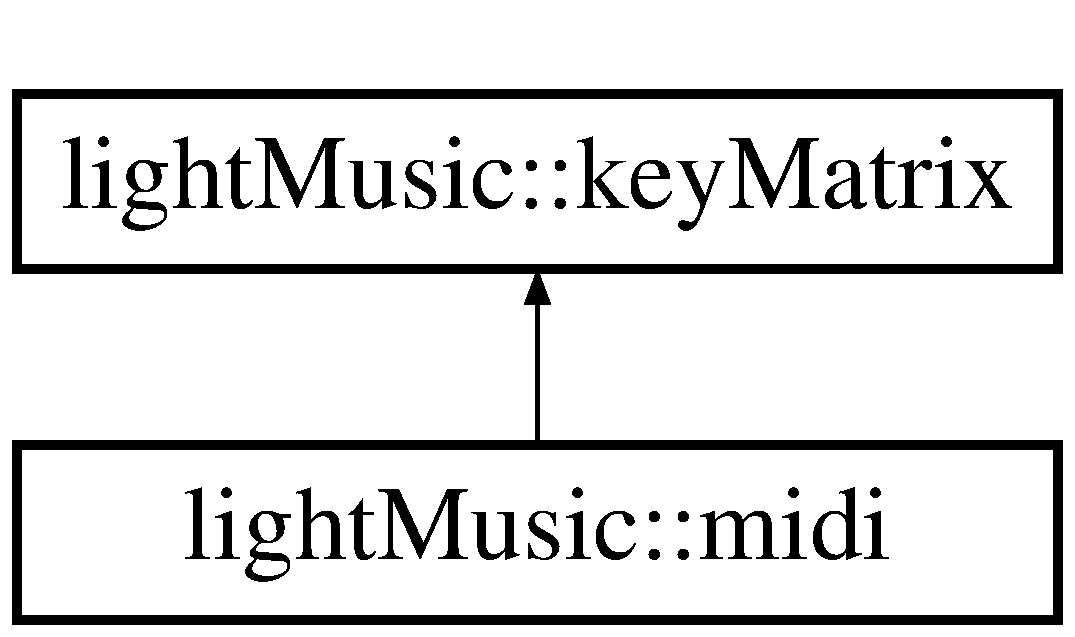
\includegraphics[height=2.000000cm]{classlight_music_1_1midi}
\end{center}
\end{figure}
\subsection*{Public Member Functions}
\begin{DoxyCompactItemize}
\item 
\hyperlink{classlight_music_1_1midi_a07cce4974be1f6bc22238c15cdba5867}{midi} (hwlib\+::target\+::pin\+\_\+in \&row1, hwlib\+::target\+::pin\+\_\+in \&row2, hwlib\+::target\+::pin\+\_\+in \&row3, hwlib\+::target\+::pin\+\_\+in \&row4, const int \&\hyperlink{classlight_music_1_1key_matrix_ab9fa44924cb5e674870f2602f92b39d3}{num\+Cols}, int \&note)
\begin{DoxyCompactList}\small\item\em Constructor. \end{DoxyCompactList}\item 
void \hyperlink{classlight_music_1_1midi_a4d5928a15254e3a087130349205a11ec}{midi\+Set\+Channel\+Bank} (hwlib\+::target\+::pin\+\_\+out \&tx\+\_\+pin, uint8\+\_\+t chan, uint8\+\_\+t bank)
\begin{DoxyCompactList}\small\item\em Set te channelbank of the vs1053. \end{DoxyCompactList}\item 
void \hyperlink{classlight_music_1_1midi_a5478f0b47275719046e67d673570f87f}{midi\+Set\+Instrument} (hwlib\+::target\+::pin\+\_\+out \&tx\+\_\+pin, uint8\+\_\+t chan, uint8\+\_\+t inst)
\begin{DoxyCompactList}\small\item\em Set te instrument of the vs1053. \end{DoxyCompactList}\item 
void \hyperlink{classlight_music_1_1midi_aa83675530bb23b24e50d1346431d2f1f}{midi\+Set\+Channel\+Volume} (hwlib\+::target\+::pin\+\_\+out \&tx\+\_\+pin, uint8\+\_\+t chan, uint8\+\_\+t vol)
\begin{DoxyCompactList}\small\item\em Set te Volume channel of the vs1053. \end{DoxyCompactList}\item 
void \hyperlink{classlight_music_1_1midi_a01bcd1c91476ac59cc6be090b2b1daef}{note\+On} (hwlib\+::target\+::pin\+\_\+out \&tx\+\_\+pin, uint8\+\_\+t chan, int row\+Ctr, int col\+Ctr, uint8\+\_\+t vel)
\begin{DoxyCompactList}\small\item\em Send midi note on message to tx\+\_\+pin. \end{DoxyCompactList}\item 
void \hyperlink{classlight_music_1_1midi_a6f47e6a388993c88f087a231a4e8f776}{note\+Off} (hwlib\+::target\+::pin\+\_\+out \&tx\+\_\+pin, uint8\+\_\+t chan, int row\+Ctr, int col\+Ctr, uint8\+\_\+t vel)
\begin{DoxyCompactList}\small\item\em Send midi note off message to tx\+\_\+pin. \end{DoxyCompactList}\item 
void \hyperlink{classlight_music_1_1midi_acc93cbd42e1d1257644f0102283b3db3}{midi\+Note\+On} (hwlib\+::target\+::pin\+\_\+out \&tx\+\_\+pin, int row\+Value\mbox{[}$\,$\mbox{]}, int col\+Ctr, uint8\+\_\+t chan, uint8\+\_\+t vel, bool key\+Pressed\mbox{[}9\mbox{]}\mbox{[}17\mbox{]})
\begin{DoxyCompactList}\small\item\em Check which button is played on keymatrix. uses \hyperlink{classlight_music_1_1midi_a01bcd1c91476ac59cc6be090b2b1daef}{note\+On()} based on the check. \end{DoxyCompactList}\item 
void \hyperlink{classlight_music_1_1midi_ae36edf372f74e28dabe879dc7600494a}{midi\+Note\+Off} (hwlib\+::target\+::pin\+\_\+out \&tx\+\_\+pin, int row\+Valu\mbox{[}$\,$\mbox{]}, int col\+Ctr, uint8\+\_\+t chan, uint8\+\_\+t vel, bool key\+Pressed\mbox{[}9\mbox{]}\mbox{[}17\mbox{]})
\begin{DoxyCompactList}\small\item\em Check which button is released on keymatrix. uses \hyperlink{classlight_music_1_1midi_a6f47e6a388993c88f087a231a4e8f776}{note\+Off()} based on the check. \end{DoxyCompactList}\item 
int \hyperlink{classlight_music_1_1midi_a8648ced30cbd9b89fb336fe874fc1102}{get\+Key\+To\+Midi\+Map} (int rowctr, int colctr)
\begin{DoxyCompactList}\small\item\em get the value of a keytomidimap on a given location \end{DoxyCompactList}\item 
uint8\+\_\+t \hyperlink{classlight_music_1_1midi_a974ccfcfc13bf4dff0743ebe7d832eed}{get\+Key\+To\+Midi\+Map8t} (int rowctr, int colctr)
\begin{DoxyCompactList}\small\item\em get the value of a keytomidimap on a given location \end{DoxyCompactList}\item 
void \hyperlink{classlight_music_1_1midi_a8ca9db5a0738b181107d2035a3439798}{min\+Max\+Velocity} (int number, bool min\+Max)
\begin{DoxyCompactList}\small\item\em set the velocity by \char`\"{}min/max number + velocity\char`\"{} \end{DoxyCompactList}\item 
int \hyperlink{classlight_music_1_1midi_aed22201e6c80c8fb8242803e22d71032}{get\+Velocity} ()
\begin{DoxyCompactList}\small\item\em get the velocity \end{DoxyCompactList}\end{DoxyCompactItemize}
\subsection*{Additional Inherited Members}


\subsection{Detailed Description}
Class to send midi messages to tx pin. 

Midi is a sub class It has six functions who makes it possible to send midi messages on the basis of the keymatrix\textquotesingle{}s input. 

\subsection{Constructor \& Destructor Documentation}
\mbox{\Hypertarget{classlight_music_1_1midi_a07cce4974be1f6bc22238c15cdba5867}\label{classlight_music_1_1midi_a07cce4974be1f6bc22238c15cdba5867}} 
\index{light\+Music\+::midi@{light\+Music\+::midi}!midi@{midi}}
\index{midi@{midi}!light\+Music\+::midi@{light\+Music\+::midi}}
\subsubsection{\texorpdfstring{midi()}{midi()}}
{\footnotesize\ttfamily light\+Music\+::midi\+::midi (\begin{DoxyParamCaption}\item[{hwlib\+::target\+::pin\+\_\+in \&}]{row1,  }\item[{hwlib\+::target\+::pin\+\_\+in \&}]{row2,  }\item[{hwlib\+::target\+::pin\+\_\+in \&}]{row3,  }\item[{hwlib\+::target\+::pin\+\_\+in \&}]{row4,  }\item[{const int \&}]{num\+Cols,  }\item[{int \&}]{note }\end{DoxyParamCaption})}



Constructor. 


\begin{DoxyParams}{Parameters}
{\em row} & $\sim$ Port of al the row inputs \\
\hline
{\em num\+\_\+cols} & $\sim$ Number of all the colums \\
\hline
{\em note} & $\sim$ Number of the first button\textquotesingle{}s key\\
\hline
\end{DoxyParams}
initialize the same parameters as the class keymatrix 

\subsection{Member Function Documentation}
\mbox{\Hypertarget{classlight_music_1_1midi_a8648ced30cbd9b89fb336fe874fc1102}\label{classlight_music_1_1midi_a8648ced30cbd9b89fb336fe874fc1102}} 
\index{light\+Music\+::midi@{light\+Music\+::midi}!get\+Key\+To\+Midi\+Map@{get\+Key\+To\+Midi\+Map}}
\index{get\+Key\+To\+Midi\+Map@{get\+Key\+To\+Midi\+Map}!light\+Music\+::midi@{light\+Music\+::midi}}
\subsubsection{\texorpdfstring{get\+Key\+To\+Midi\+Map()}{getKeyToMidiMap()}}
{\footnotesize\ttfamily int light\+Music\+::midi\+::get\+Key\+To\+Midi\+Map (\begin{DoxyParamCaption}\item[{int}]{rowctr,  }\item[{int}]{colctr }\end{DoxyParamCaption})}



get the value of a keytomidimap on a given location 


\begin{DoxyParams}{Parameters}
{\em rowctr} & which row \\
\hline
{\em colctr} & which column \\
\hline
\end{DoxyParams}
\begin{DoxyReturn}{Returns}
int of the key on the given location 
\end{DoxyReturn}
\mbox{\Hypertarget{classlight_music_1_1midi_a974ccfcfc13bf4dff0743ebe7d832eed}\label{classlight_music_1_1midi_a974ccfcfc13bf4dff0743ebe7d832eed}} 
\index{light\+Music\+::midi@{light\+Music\+::midi}!get\+Key\+To\+Midi\+Map8t@{get\+Key\+To\+Midi\+Map8t}}
\index{get\+Key\+To\+Midi\+Map8t@{get\+Key\+To\+Midi\+Map8t}!light\+Music\+::midi@{light\+Music\+::midi}}
\subsubsection{\texorpdfstring{get\+Key\+To\+Midi\+Map8t()}{getKeyToMidiMap8t()}}
{\footnotesize\ttfamily uint8\+\_\+t light\+Music\+::midi\+::get\+Key\+To\+Midi\+Map8t (\begin{DoxyParamCaption}\item[{int}]{rowctr,  }\item[{int}]{colctr }\end{DoxyParamCaption})}



get the value of a keytomidimap on a given location 


\begin{DoxyParams}{Parameters}
{\em rowctr} & which row \\
\hline
{\em colctr} & which column \\
\hline
\end{DoxyParams}
\begin{DoxyReturn}{Returns}
uint8\+\_\+t of the key on the given location 
\end{DoxyReturn}
\mbox{\Hypertarget{classlight_music_1_1midi_aed22201e6c80c8fb8242803e22d71032}\label{classlight_music_1_1midi_aed22201e6c80c8fb8242803e22d71032}} 
\index{light\+Music\+::midi@{light\+Music\+::midi}!get\+Velocity@{get\+Velocity}}
\index{get\+Velocity@{get\+Velocity}!light\+Music\+::midi@{light\+Music\+::midi}}
\subsubsection{\texorpdfstring{get\+Velocity()}{getVelocity()}}
{\footnotesize\ttfamily int light\+Music\+::midi\+::get\+Velocity (\begin{DoxyParamCaption}{ }\end{DoxyParamCaption})}



get the velocity 

\begin{DoxyReturn}{Returns}
int velocity 
\end{DoxyReturn}
\mbox{\Hypertarget{classlight_music_1_1midi_ae36edf372f74e28dabe879dc7600494a}\label{classlight_music_1_1midi_ae36edf372f74e28dabe879dc7600494a}} 
\index{light\+Music\+::midi@{light\+Music\+::midi}!midi\+Note\+Off@{midi\+Note\+Off}}
\index{midi\+Note\+Off@{midi\+Note\+Off}!light\+Music\+::midi@{light\+Music\+::midi}}
\subsubsection{\texorpdfstring{midi\+Note\+Off()}{midiNoteOff()}}
{\footnotesize\ttfamily void light\+Music\+::midi\+::midi\+Note\+Off (\begin{DoxyParamCaption}\item[{hwlib\+::target\+::pin\+\_\+out \&}]{tx\+\_\+pin,  }\item[{int}]{row\+Valu\mbox{[}$\,$\mbox{]},  }\item[{int}]{col\+Ctr,  }\item[{uint8\+\_\+t}]{chan,  }\item[{uint8\+\_\+t}]{vel,  }\item[{bool}]{key\+Pressed\mbox{[}9\mbox{]}\mbox{[}17\mbox{]} }\end{DoxyParamCaption})}



Check which button is released on keymatrix. uses \hyperlink{classlight_music_1_1midi_a6f47e6a388993c88f087a231a4e8f776}{note\+Off()} based on the check. 


\begin{DoxyParams}{Parameters}
{\em tx\+\_\+pin} & $\sim$ The pin on which sends midi messages \\
\hline
{\em row\+Value} & $\sim$ Array with the values of the row \\
\hline
{\em col\+Ctr} & $\sim$ Container who holds the released col number \\
\hline
{\em chan} & $\sim$ Uint8\+\_\+t to send midi on a specific channel \\
\hline
{\em vel} & $\sim$ veloctity \\
\hline
\end{DoxyParams}
\mbox{\Hypertarget{classlight_music_1_1midi_acc93cbd42e1d1257644f0102283b3db3}\label{classlight_music_1_1midi_acc93cbd42e1d1257644f0102283b3db3}} 
\index{light\+Music\+::midi@{light\+Music\+::midi}!midi\+Note\+On@{midi\+Note\+On}}
\index{midi\+Note\+On@{midi\+Note\+On}!light\+Music\+::midi@{light\+Music\+::midi}}
\subsubsection{\texorpdfstring{midi\+Note\+On()}{midiNoteOn()}}
{\footnotesize\ttfamily void light\+Music\+::midi\+::midi\+Note\+On (\begin{DoxyParamCaption}\item[{hwlib\+::target\+::pin\+\_\+out \&}]{tx\+\_\+pin,  }\item[{int}]{row\+Value\mbox{[}$\,$\mbox{]},  }\item[{int}]{col\+Ctr,  }\item[{uint8\+\_\+t}]{chan,  }\item[{uint8\+\_\+t}]{vel,  }\item[{bool}]{key\+Pressed\mbox{[}9\mbox{]}\mbox{[}17\mbox{]} }\end{DoxyParamCaption})}



Check which button is played on keymatrix. uses \hyperlink{classlight_music_1_1midi_a01bcd1c91476ac59cc6be090b2b1daef}{note\+On()} based on the check. 


\begin{DoxyParams}{Parameters}
{\em tx\+\_\+pin} & $\sim$ The pin on which sends midi messages \\
\hline
{\em row\+Value} & $\sim$ Array with the values of the row \\
\hline
{\em col\+Ctr} & $\sim$ Container who holds the released col number \\
\hline
{\em chan} & $\sim$ Uint8\+\_\+t to send midi on a specific channel \\
\hline
{\em vel} & $\sim$ veloctity \\
\hline
\end{DoxyParams}
\mbox{\Hypertarget{classlight_music_1_1midi_a4d5928a15254e3a087130349205a11ec}\label{classlight_music_1_1midi_a4d5928a15254e3a087130349205a11ec}} 
\index{light\+Music\+::midi@{light\+Music\+::midi}!midi\+Set\+Channel\+Bank@{midi\+Set\+Channel\+Bank}}
\index{midi\+Set\+Channel\+Bank@{midi\+Set\+Channel\+Bank}!light\+Music\+::midi@{light\+Music\+::midi}}
\subsubsection{\texorpdfstring{midi\+Set\+Channel\+Bank()}{midiSetChannelBank()}}
{\footnotesize\ttfamily void light\+Music\+::midi\+::midi\+Set\+Channel\+Bank (\begin{DoxyParamCaption}\item[{hwlib\+::target\+::pin\+\_\+out \&}]{tx\+\_\+pin,  }\item[{uint8\+\_\+t}]{chan,  }\item[{uint8\+\_\+t}]{bank }\end{DoxyParamCaption})}



Set te channelbank of the vs1053. 


\begin{DoxyParams}{Parameters}
{\em tx\+\_\+pin} & $\sim$ The pin on which sends midi messages \\
\hline
{\em chan} & $\sim$ Channel \\
\hline
{\em bank} & $\sim$ Bank \\
\hline
\end{DoxyParams}
\mbox{\Hypertarget{classlight_music_1_1midi_aa83675530bb23b24e50d1346431d2f1f}\label{classlight_music_1_1midi_aa83675530bb23b24e50d1346431d2f1f}} 
\index{light\+Music\+::midi@{light\+Music\+::midi}!midi\+Set\+Channel\+Volume@{midi\+Set\+Channel\+Volume}}
\index{midi\+Set\+Channel\+Volume@{midi\+Set\+Channel\+Volume}!light\+Music\+::midi@{light\+Music\+::midi}}
\subsubsection{\texorpdfstring{midi\+Set\+Channel\+Volume()}{midiSetChannelVolume()}}
{\footnotesize\ttfamily void light\+Music\+::midi\+::midi\+Set\+Channel\+Volume (\begin{DoxyParamCaption}\item[{hwlib\+::target\+::pin\+\_\+out \&}]{tx\+\_\+pin,  }\item[{uint8\+\_\+t}]{chan,  }\item[{uint8\+\_\+t}]{vol }\end{DoxyParamCaption})}



Set te Volume channel of the vs1053. 


\begin{DoxyParams}{Parameters}
{\em tx\+\_\+pin} & $\sim$ The pin on which sends midi messages \\
\hline
{\em chan} & $\sim$ Channel \\
\hline
{\em vol} & $\sim$ volume \\
\hline
\end{DoxyParams}
\mbox{\Hypertarget{classlight_music_1_1midi_a5478f0b47275719046e67d673570f87f}\label{classlight_music_1_1midi_a5478f0b47275719046e67d673570f87f}} 
\index{light\+Music\+::midi@{light\+Music\+::midi}!midi\+Set\+Instrument@{midi\+Set\+Instrument}}
\index{midi\+Set\+Instrument@{midi\+Set\+Instrument}!light\+Music\+::midi@{light\+Music\+::midi}}
\subsubsection{\texorpdfstring{midi\+Set\+Instrument()}{midiSetInstrument()}}
{\footnotesize\ttfamily void light\+Music\+::midi\+::midi\+Set\+Instrument (\begin{DoxyParamCaption}\item[{hwlib\+::target\+::pin\+\_\+out \&}]{tx\+\_\+pin,  }\item[{uint8\+\_\+t}]{chan,  }\item[{uint8\+\_\+t}]{inst }\end{DoxyParamCaption})}



Set te instrument of the vs1053. 


\begin{DoxyParams}{Parameters}
{\em tx\+\_\+pin} & $\sim$ The pin on which sends midi messages \\
\hline
{\em chan} & $\sim$ Channel \\
\hline
{\em inst} & $\sim$ Instrument \\
\hline
\end{DoxyParams}
\mbox{\Hypertarget{classlight_music_1_1midi_a8ca9db5a0738b181107d2035a3439798}\label{classlight_music_1_1midi_a8ca9db5a0738b181107d2035a3439798}} 
\index{light\+Music\+::midi@{light\+Music\+::midi}!min\+Max\+Velocity@{min\+Max\+Velocity}}
\index{min\+Max\+Velocity@{min\+Max\+Velocity}!light\+Music\+::midi@{light\+Music\+::midi}}
\subsubsection{\texorpdfstring{min\+Max\+Velocity()}{minMaxVelocity()}}
{\footnotesize\ttfamily void light\+Music\+::midi\+::min\+Max\+Velocity (\begin{DoxyParamCaption}\item[{int}]{number,  }\item[{bool}]{min\+Max }\end{DoxyParamCaption})}



set the velocity by \char`\"{}min/max number + velocity\char`\"{} 


\begin{DoxyParams}{Parameters}
{\em number} & how many numbers it wil change \\
\hline
{\em min\+Max} & minus(false) or plus(true) \\
\hline
\end{DoxyParams}
\mbox{\Hypertarget{classlight_music_1_1midi_a6f47e6a388993c88f087a231a4e8f776}\label{classlight_music_1_1midi_a6f47e6a388993c88f087a231a4e8f776}} 
\index{light\+Music\+::midi@{light\+Music\+::midi}!note\+Off@{note\+Off}}
\index{note\+Off@{note\+Off}!light\+Music\+::midi@{light\+Music\+::midi}}
\subsubsection{\texorpdfstring{note\+Off()}{noteOff()}}
{\footnotesize\ttfamily void light\+Music\+::midi\+::note\+Off (\begin{DoxyParamCaption}\item[{hwlib\+::target\+::pin\+\_\+out \&}]{tx\+\_\+pin,  }\item[{uint8\+\_\+t}]{chan,  }\item[{int}]{row\+Ctr,  }\item[{int}]{col\+Ctr,  }\item[{uint8\+\_\+t}]{vel }\end{DoxyParamCaption})}



Send midi note off message to tx\+\_\+pin. 


\begin{DoxyParams}{Parameters}
{\em tx\+\_\+pin} & $\sim$ The pin on which sends midi messages \\
\hline
{\em chan} & $\sim$ Uint8\+\_\+t to send midi on a specific channel \\
\hline
{\em row\+Ctr} & $\sim$ Container who holds the released row number \\
\hline
{\em col\+Ctr} & $\sim$ Container who holds the released col number \\
\hline
{\em vel} & $\sim$ velocity \\
\hline
\end{DoxyParams}
\mbox{\Hypertarget{classlight_music_1_1midi_a01bcd1c91476ac59cc6be090b2b1daef}\label{classlight_music_1_1midi_a01bcd1c91476ac59cc6be090b2b1daef}} 
\index{light\+Music\+::midi@{light\+Music\+::midi}!note\+On@{note\+On}}
\index{note\+On@{note\+On}!light\+Music\+::midi@{light\+Music\+::midi}}
\subsubsection{\texorpdfstring{note\+On()}{noteOn()}}
{\footnotesize\ttfamily void light\+Music\+::midi\+::note\+On (\begin{DoxyParamCaption}\item[{hwlib\+::target\+::pin\+\_\+out \&}]{tx\+\_\+pin,  }\item[{uint8\+\_\+t}]{chan,  }\item[{int}]{row\+Ctr,  }\item[{int}]{col\+Ctr,  }\item[{uint8\+\_\+t}]{vel }\end{DoxyParamCaption})}



Send midi note on message to tx\+\_\+pin. 


\begin{DoxyParams}{Parameters}
{\em tx\+\_\+pin} & $\sim$ The pin on which sends midi messages \\
\hline
{\em chan} & $\sim$ Uint8\+\_\+t to send midi on a specific channel \\
\hline
{\em row\+Ctr} & $\sim$ Container who holds the pressed row number \\
\hline
{\em col\+Ctr} & $\sim$ Container who holds the pressed col number \\
\hline
{\em vel} & $\sim$ velocity \\
\hline
\end{DoxyParams}


The documentation for this class was generated from the following files\+:\begin{DoxyCompactItemize}
\item 
C\+:/ti-\/software/lightmusic/lightmusic/midi.\+hpp\item 
C\+:/ti-\/software/lightmusic/lightmusic/midi.\+cpp\end{DoxyCompactItemize}

\chapter{File Documentation}
\hypertarget{constants8x8chars_8hpp}{}\section{C\+:/ti-\/software/lightmusic/lightmusic/constants8x8chars.hpp File Reference}
\label{constants8x8chars_8hpp}\index{C\+:/ti-\/software/lightmusic/lightmusic/constants8x8chars.\+hpp@{C\+:/ti-\/software/lightmusic/lightmusic/constants8x8chars.\+hpp}}
{\ttfamily \#include \char`\"{}stdint.\+h\char`\"{}}\newline
\subsection*{Variables}
\begin{DoxyCompactItemize}
\item 
\mbox{\Hypertarget{constants8x8chars_8hpp_a8f67b94ef5dbb12836e0a6655f00e262}\label{constants8x8chars_8hpp_a8f67b94ef5dbb12836e0a6655f00e262}} 
constexpr int \hyperlink{constants8x8chars_8hpp_a8f67b94ef5dbb12836e0a6655f00e262}{const8x8\+Ch\+::\+L\+E\+T\+T\+E\+RS} \mbox{[}12\mbox{]}\mbox{[}9\mbox{]}\mbox{[}9\mbox{]}
\begin{DoxyCompactList}\small\item\em L\+E\+T\+T\+E\+RS -\/ all the letters of the keys on a piano included sharp C-\/B. \end{DoxyCompactList}\item 
\mbox{\Hypertarget{constants8x8chars_8hpp_a05860dae5611e4470acb993fde59b134}\label{constants8x8chars_8hpp_a05860dae5611e4470acb993fde59b134}} 
constexpr int \hyperlink{constants8x8chars_8hpp_a05860dae5611e4470acb993fde59b134}{const8x8\+Ch\+::\+N\+U\+M\+B\+E\+RS} \mbox{[}10\mbox{]}\mbox{[}9\mbox{]}\mbox{[}9\mbox{]}
\begin{DoxyCompactList}\small\item\em N\+U\+M\+B\+E\+RS -\/ all the numbers 0-\/9. \end{DoxyCompactList}\item 
\mbox{\Hypertarget{constants8x8chars_8hpp_a4d935ac6acdfd2dbc1a0d5171c2a6d64}\label{constants8x8chars_8hpp_a4d935ac6acdfd2dbc1a0d5171c2a6d64}} 
constexpr int \hyperlink{constants8x8chars_8hpp_a4d935ac6acdfd2dbc1a0d5171c2a6d64}{const8x8\+Ch\+::\+S\+P\+A\+C\+E\+M\+X\+IN} \mbox{[}5\mbox{]}\mbox{[}9\mbox{]}\mbox{[}9\mbox{]}
\begin{DoxyCompactList}\small\item\em M\+X\+IN -\/ The letters to write min or max with a \char`\"{}space\char`\"{} (S\+P\+A\+CE, M, X, I, N). \end{DoxyCompactList}\end{DoxyCompactItemize}

\hypertarget{constantsmax7219_8hpp}{}\section{C\+:/ti-\/software/lightmusic/lightmusic/constantsmax7219.hpp File Reference}
\label{constantsmax7219_8hpp}\index{C\+:/ti-\/software/lightmusic/lightmusic/constantsmax7219.\+hpp@{C\+:/ti-\/software/lightmusic/lightmusic/constantsmax7219.\+hpp}}
{\ttfamily \#include \char`\"{}stdint.\+h\char`\"{}}\newline
\subsection*{Variables}
\begin{DoxyCompactItemize}
\item 
constexpr uint8\+\_\+t \hyperlink{constantsmax7219_8hpp_aac7978b5e88ce54d4caa5decb1f1ce0d}{const\+Max7219\+::\+M\+A\+X7219\+\_\+\+R\+E\+G\+\_\+\+N\+O\+\_\+\+OP} = 0x00
\item 
constexpr uint8\+\_\+t \hyperlink{constantsmax7219_8hpp_a6c4cdf1cbbdcf59e4f0047b3d417d188}{const\+Max7219\+::\+M\+A\+X7219\+\_\+\+R\+E\+G\+\_\+\+D\+I\+G\+I\+T1} = 0x01
\item 
\mbox{\Hypertarget{constantsmax7219_8hpp_a59aa558613b8a572caa77325b1412d24}\label{constantsmax7219_8hpp_a59aa558613b8a572caa77325b1412d24}} 
constexpr uint8\+\_\+t {\bfseries const\+Max7219\+::\+M\+A\+X7219\+\_\+\+R\+E\+G\+\_\+\+D\+I\+G\+I\+T2} = 0x02
\item 
\mbox{\Hypertarget{constantsmax7219_8hpp_adc671a197fcc9987103303a996f01d43}\label{constantsmax7219_8hpp_adc671a197fcc9987103303a996f01d43}} 
constexpr uint8\+\_\+t {\bfseries const\+Max7219\+::\+M\+A\+X7219\+\_\+\+R\+E\+G\+\_\+\+D\+I\+G\+I\+T3} = 0x03
\item 
\mbox{\Hypertarget{constantsmax7219_8hpp_af5d4702e3b3dfae39d58db045914f097}\label{constantsmax7219_8hpp_af5d4702e3b3dfae39d58db045914f097}} 
constexpr uint8\+\_\+t {\bfseries const\+Max7219\+::\+M\+A\+X7219\+\_\+\+R\+E\+G\+\_\+\+D\+I\+G\+I\+T4} = 0x04
\item 
\mbox{\Hypertarget{constantsmax7219_8hpp_ad02aaf0bbb0b8c26aa1d7c33ecd4d05f}\label{constantsmax7219_8hpp_ad02aaf0bbb0b8c26aa1d7c33ecd4d05f}} 
constexpr uint8\+\_\+t {\bfseries const\+Max7219\+::\+M\+A\+X7219\+\_\+\+R\+E\+G\+\_\+\+D\+I\+G\+I\+T5} = 0x05
\item 
\mbox{\Hypertarget{constantsmax7219_8hpp_a61c25354925402d22431cf7993ef47bc}\label{constantsmax7219_8hpp_a61c25354925402d22431cf7993ef47bc}} 
constexpr uint8\+\_\+t {\bfseries const\+Max7219\+::\+M\+A\+X7219\+\_\+\+R\+E\+G\+\_\+\+D\+I\+G\+I\+T6} = 0x06
\item 
\mbox{\Hypertarget{constantsmax7219_8hpp_a40541e619f19d61fcd7be58a128c9b53}\label{constantsmax7219_8hpp_a40541e619f19d61fcd7be58a128c9b53}} 
constexpr uint8\+\_\+t {\bfseries const\+Max7219\+::\+M\+A\+X7219\+\_\+\+R\+E\+G\+\_\+\+D\+I\+G\+I\+T7} = 0x07
\item 
\mbox{\Hypertarget{constantsmax7219_8hpp_ae0d80a121ec9a710573f2ae33346d42f}\label{constantsmax7219_8hpp_ae0d80a121ec9a710573f2ae33346d42f}} 
constexpr uint8\+\_\+t {\bfseries const\+Max7219\+::\+M\+A\+X7219\+\_\+\+R\+E\+G\+\_\+\+D\+I\+G\+I\+T8} = 0x08
\item 
constexpr uint8\+\_\+t \hyperlink{constantsmax7219_8hpp_aa9860c46c595104fd7c28fa6e9065af6}{const\+Max7219\+::\+M\+A\+X7219\+\_\+\+R\+E\+G\+\_\+\+D\+E\+C\+O\+DE} = 0x09
\item 
\mbox{\Hypertarget{constantsmax7219_8hpp_a00a7e1d1bb1ae5e44333ef33a3b0cd0b}\label{constantsmax7219_8hpp_a00a7e1d1bb1ae5e44333ef33a3b0cd0b}} 
constexpr uint8\+\_\+t {\bfseries const\+Max7219\+::\+M\+A\+X7219\+\_\+\+R\+E\+G\+\_\+\+I\+N\+T\+E\+N\+S\+I\+TY} = 0x0A
\item 
\mbox{\Hypertarget{constantsmax7219_8hpp_a3d7c24a5efb28a9741ed901badf7ac83}\label{constantsmax7219_8hpp_a3d7c24a5efb28a9741ed901badf7ac83}} 
constexpr uint8\+\_\+t {\bfseries const\+Max7219\+::\+M\+A\+X7219\+\_\+\+R\+E\+G\+\_\+\+S\+C\+A\+N\+\_\+\+L\+I\+M\+IT} = 0x0B
\item 
\mbox{\Hypertarget{constantsmax7219_8hpp_a566dd9032791944f3ff5ef57c4ee04a3}\label{constantsmax7219_8hpp_a566dd9032791944f3ff5ef57c4ee04a3}} 
constexpr uint8\+\_\+t {\bfseries const\+Max7219\+::\+M\+A\+X7219\+\_\+\+R\+E\+G\+\_\+\+S\+H\+U\+T\+D\+O\+WN} = 0x0C
\item 
\mbox{\Hypertarget{constantsmax7219_8hpp_af09e36ac4f556db83d8dd27f7a58911a}\label{constantsmax7219_8hpp_af09e36ac4f556db83d8dd27f7a58911a}} 
constexpr uint8\+\_\+t {\bfseries const\+Max7219\+::\+M\+A\+X7219\+\_\+\+R\+E\+G\+\_\+\+D\+I\+S\+P\+L\+A\+Y\+T\+E\+ST} = 0x0F
\item 
constexpr uint8\+\_\+t \hyperlink{constantsmax7219_8hpp_a6e8f42c82acd0ac2e44b122358022d47}{const\+Max7219\+::\+M\+A\+X7219\+\_\+\+D\+A\+T\+A\+\_\+\+D\+E\+C\+O\+D\+E\+\_\+\+N\+O\+\_\+\+D\+E\+C\+O\+DE} = 0x00
\item 
\mbox{\Hypertarget{constantsmax7219_8hpp_ab2e70b36022062d77edb252451c515a0}\label{constantsmax7219_8hpp_ab2e70b36022062d77edb252451c515a0}} 
constexpr uint8\+\_\+t {\bfseries const\+Max7219\+::\+M\+A\+X7219\+\_\+\+D\+A\+T\+A\+\_\+\+D\+E\+C\+O\+D\+E\+\_\+\+C\+O\+D\+E\+\_\+\+B1} = 0x01
\item 
\mbox{\Hypertarget{constantsmax7219_8hpp_ae55d550fd6cb4ba65acd63e0a07069d1}\label{constantsmax7219_8hpp_ae55d550fd6cb4ba65acd63e0a07069d1}} 
constexpr uint8\+\_\+t {\bfseries const\+Max7219\+::\+M\+A\+X7219\+\_\+\+D\+A\+T\+A\+\_\+\+D\+E\+C\+O\+D\+E\+\_\+\+C\+O\+D\+E\+\_\+\+B2} = 0x0F
\item 
\mbox{\Hypertarget{constantsmax7219_8hpp_ad579a3beeeb9154f6e606494bdf743de}\label{constantsmax7219_8hpp_ad579a3beeeb9154f6e606494bdf743de}} 
constexpr uint8\+\_\+t {\bfseries const\+Max7219\+::\+M\+A\+X7219\+\_\+\+D\+A\+T\+A\+\_\+\+D\+E\+C\+O\+D\+E\+\_\+\+C\+O\+D\+E\+\_\+\+B\+\_\+\+A\+LL} = 0x\+FF
\item 
\mbox{\Hypertarget{constantsmax7219_8hpp_aa351ffcad84400ee1076c4e5612d0af2}\label{constantsmax7219_8hpp_aa351ffcad84400ee1076c4e5612d0af2}} 
constexpr uint8\+\_\+t \hyperlink{constantsmax7219_8hpp_aa351ffcad84400ee1076c4e5612d0af2}{const\+Max7219\+::\+M\+A\+X7219\+\_\+\+D\+A\+T\+A\+\_\+\+I\+N\+T\+E\+N\+S\+I\+T\+Y\+\_\+\+L\+V\+L1} = 0x00
\begin{DoxyCompactList}\small\item\em I\+N\+T\+E\+N\+S\+I\+TY register data -\/ control the display brightness. \end{DoxyCompactList}\item 
\mbox{\Hypertarget{constantsmax7219_8hpp_aafb7276ccf357b1c133dfb427f211989}\label{constantsmax7219_8hpp_aafb7276ccf357b1c133dfb427f211989}} 
constexpr uint8\+\_\+t {\bfseries const\+Max7219\+::\+M\+A\+X7219\+\_\+\+D\+A\+T\+A\+\_\+\+I\+N\+T\+E\+N\+S\+I\+T\+Y\+\_\+\+L\+V\+L2} = 0x01
\item 
\mbox{\Hypertarget{constantsmax7219_8hpp_a2c69fb3e61763ed8a9a8188e5539d737}\label{constantsmax7219_8hpp_a2c69fb3e61763ed8a9a8188e5539d737}} 
constexpr uint8\+\_\+t {\bfseries const\+Max7219\+::\+M\+A\+X7219\+\_\+\+D\+A\+T\+A\+\_\+\+I\+N\+T\+E\+N\+S\+I\+T\+Y\+\_\+\+L\+V\+L3} = 0x02
\item 
\mbox{\Hypertarget{constantsmax7219_8hpp_a5d37066ce3fe2238d896b0058f4e5b4d}\label{constantsmax7219_8hpp_a5d37066ce3fe2238d896b0058f4e5b4d}} 
constexpr uint8\+\_\+t {\bfseries const\+Max7219\+::\+M\+A\+X7219\+\_\+\+D\+A\+T\+A\+\_\+\+I\+N\+T\+E\+N\+S\+I\+T\+Y\+\_\+\+L\+V\+L4} = 0x03
\item 
\mbox{\Hypertarget{constantsmax7219_8hpp_abda032ca5cc591ce3a80d49d80ec0fad}\label{constantsmax7219_8hpp_abda032ca5cc591ce3a80d49d80ec0fad}} 
constexpr uint8\+\_\+t {\bfseries const\+Max7219\+::\+M\+A\+X7219\+\_\+\+D\+A\+T\+A\+\_\+\+I\+N\+T\+E\+N\+S\+I\+T\+Y\+\_\+\+L\+V\+L5} = 0x04
\item 
\mbox{\Hypertarget{constantsmax7219_8hpp_a4974ccb84b71eb4a47eb21b47b38fc26}\label{constantsmax7219_8hpp_a4974ccb84b71eb4a47eb21b47b38fc26}} 
constexpr uint8\+\_\+t {\bfseries const\+Max7219\+::\+M\+A\+X7219\+\_\+\+D\+A\+T\+A\+\_\+\+I\+N\+T\+E\+N\+S\+I\+T\+Y\+\_\+\+L\+V\+L6} = 0x05
\item 
\mbox{\Hypertarget{constantsmax7219_8hpp_a3e08bb9545c153f71ad89a178165fc41}\label{constantsmax7219_8hpp_a3e08bb9545c153f71ad89a178165fc41}} 
constexpr uint8\+\_\+t {\bfseries const\+Max7219\+::\+M\+A\+X7219\+\_\+\+D\+A\+T\+A\+\_\+\+I\+N\+T\+E\+N\+S\+I\+T\+Y\+\_\+\+L\+V\+L7} = 0x06
\item 
\mbox{\Hypertarget{constantsmax7219_8hpp_a0b70cfff51cd5fecbd6f221ee89d1f42}\label{constantsmax7219_8hpp_a0b70cfff51cd5fecbd6f221ee89d1f42}} 
constexpr uint8\+\_\+t {\bfseries const\+Max7219\+::\+M\+A\+X7219\+\_\+\+D\+A\+T\+A\+\_\+\+I\+N\+T\+E\+N\+S\+I\+T\+Y\+\_\+\+L\+V\+L8} = 0x07
\item 
\mbox{\Hypertarget{constantsmax7219_8hpp_a6be6a63cacf66ecbabff97b574bcb953}\label{constantsmax7219_8hpp_a6be6a63cacf66ecbabff97b574bcb953}} 
constexpr uint8\+\_\+t {\bfseries const\+Max7219\+::\+M\+A\+X7219\+\_\+\+D\+A\+T\+A\+\_\+\+I\+N\+T\+E\+N\+S\+I\+T\+Y\+\_\+\+L\+V\+L9} = 0x08
\item 
\mbox{\Hypertarget{constantsmax7219_8hpp_aa5cae95440012b8a24af036ea0f0c4fb}\label{constantsmax7219_8hpp_aa5cae95440012b8a24af036ea0f0c4fb}} 
constexpr uint8\+\_\+t {\bfseries const\+Max7219\+::\+M\+A\+X7219\+\_\+\+D\+A\+T\+A\+\_\+\+I\+N\+T\+E\+N\+S\+I\+T\+Y\+\_\+\+L\+V\+L10} = 0x09
\item 
\mbox{\Hypertarget{constantsmax7219_8hpp_af4e7d660b8e143af1639a4c45a6bdaa5}\label{constantsmax7219_8hpp_af4e7d660b8e143af1639a4c45a6bdaa5}} 
constexpr uint8\+\_\+t {\bfseries const\+Max7219\+::\+M\+A\+X7219\+\_\+\+D\+A\+T\+A\+\_\+\+I\+N\+T\+E\+N\+S\+I\+T\+Y\+\_\+\+L\+V\+L11} = 0x0A
\item 
\mbox{\Hypertarget{constantsmax7219_8hpp_a19e2fe544305211e62d39cc1a61e21b0}\label{constantsmax7219_8hpp_a19e2fe544305211e62d39cc1a61e21b0}} 
constexpr uint8\+\_\+t {\bfseries const\+Max7219\+::\+M\+A\+X7219\+\_\+\+D\+A\+T\+A\+\_\+\+I\+N\+T\+E\+N\+S\+I\+T\+Y\+\_\+\+L\+V\+L12} = 0x0B
\item 
\mbox{\Hypertarget{constantsmax7219_8hpp_aac25082d98a989187919a809736f387a}\label{constantsmax7219_8hpp_aac25082d98a989187919a809736f387a}} 
constexpr uint8\+\_\+t {\bfseries const\+Max7219\+::\+M\+A\+X7219\+\_\+\+D\+A\+T\+A\+\_\+\+I\+N\+T\+E\+N\+S\+I\+T\+Y\+\_\+\+L\+V\+L13} = 0x0C
\item 
\mbox{\Hypertarget{constantsmax7219_8hpp_a0c537ee30777415d70e3341d7b00d96a}\label{constantsmax7219_8hpp_a0c537ee30777415d70e3341d7b00d96a}} 
constexpr uint8\+\_\+t {\bfseries const\+Max7219\+::\+M\+A\+X7219\+\_\+\+D\+A\+T\+A\+\_\+\+I\+N\+T\+E\+N\+S\+I\+T\+Y\+\_\+\+L\+V\+L14} = 0x0D
\item 
\mbox{\Hypertarget{constantsmax7219_8hpp_a27c951cd2bcc9b88b9c214e7d839f32d}\label{constantsmax7219_8hpp_a27c951cd2bcc9b88b9c214e7d839f32d}} 
constexpr uint8\+\_\+t {\bfseries const\+Max7219\+::\+M\+A\+X7219\+\_\+\+D\+A\+T\+A\+\_\+\+I\+N\+T\+E\+N\+S\+I\+T\+Y\+\_\+\+L\+V\+L15} = 0x0E
\item 
\mbox{\Hypertarget{constantsmax7219_8hpp_ae9fdd340085628e19f2c012c0d17253c}\label{constantsmax7219_8hpp_ae9fdd340085628e19f2c012c0d17253c}} 
constexpr uint8\+\_\+t {\bfseries const\+Max7219\+::\+M\+A\+X7219\+\_\+\+D\+A\+T\+A\+\_\+\+I\+N\+T\+E\+N\+S\+I\+T\+Y\+\_\+\+L\+V\+L16} = 0x0F
\item 
\mbox{\Hypertarget{constantsmax7219_8hpp_ac54731355472b7ae62749e7ecc54eeb8}\label{constantsmax7219_8hpp_ac54731355472b7ae62749e7ecc54eeb8}} 
constexpr uint8\+\_\+t \hyperlink{constantsmax7219_8hpp_ac54731355472b7ae62749e7ecc54eeb8}{const\+Max7219\+::\+M\+A\+X7219\+\_\+\+D\+A\+T\+A\+\_\+\+S\+C\+A\+N\+\_\+\+L\+I\+M\+I\+T1} = 0x00
\begin{DoxyCompactList}\small\item\em S\+C\+AN L\+I\+M\+IT register data -\/ sets how many digits are displayed, from 1 to 8. \end{DoxyCompactList}\item 
\mbox{\Hypertarget{constantsmax7219_8hpp_a4142374604d732c988de42ce08091cd1}\label{constantsmax7219_8hpp_a4142374604d732c988de42ce08091cd1}} 
constexpr uint8\+\_\+t {\bfseries const\+Max7219\+::\+M\+A\+X7219\+\_\+\+D\+A\+T\+A\+\_\+\+S\+C\+A\+N\+\_\+\+L\+I\+M\+I\+T2} = 0x01
\item 
\mbox{\Hypertarget{constantsmax7219_8hpp_ad3843d2b9a1799fce55c089345f02e00}\label{constantsmax7219_8hpp_ad3843d2b9a1799fce55c089345f02e00}} 
constexpr uint8\+\_\+t {\bfseries const\+Max7219\+::\+M\+A\+X7219\+\_\+\+D\+A\+T\+A\+\_\+\+S\+C\+A\+N\+\_\+\+L\+I\+M\+I\+T3} = 0x02
\item 
\mbox{\Hypertarget{constantsmax7219_8hpp_a051e381eef51aee89b909f3073b903c2}\label{constantsmax7219_8hpp_a051e381eef51aee89b909f3073b903c2}} 
constexpr uint8\+\_\+t {\bfseries const\+Max7219\+::\+M\+A\+X7219\+\_\+\+D\+A\+T\+A\+\_\+\+S\+C\+A\+N\+\_\+\+L\+I\+M\+I\+T4} = 0x03
\item 
\mbox{\Hypertarget{constantsmax7219_8hpp_a33088ac74a8e741a054f8fcb332c3b9b}\label{constantsmax7219_8hpp_a33088ac74a8e741a054f8fcb332c3b9b}} 
constexpr uint8\+\_\+t {\bfseries const\+Max7219\+::\+M\+A\+X7219\+\_\+\+D\+A\+T\+A\+\_\+\+S\+C\+A\+N\+\_\+\+L\+I\+M\+I\+T5} = 0x04
\item 
\mbox{\Hypertarget{constantsmax7219_8hpp_abd5b8192ca5e22337e9c577e452169af}\label{constantsmax7219_8hpp_abd5b8192ca5e22337e9c577e452169af}} 
constexpr uint8\+\_\+t {\bfseries const\+Max7219\+::\+M\+A\+X7219\+\_\+\+D\+A\+T\+A\+\_\+\+S\+C\+A\+N\+\_\+\+L\+I\+M\+I\+T6} = 0x05
\item 
\mbox{\Hypertarget{constantsmax7219_8hpp_ab542e354dfb6d98fb8e8949c6b75d13d}\label{constantsmax7219_8hpp_ab542e354dfb6d98fb8e8949c6b75d13d}} 
constexpr uint8\+\_\+t {\bfseries const\+Max7219\+::\+M\+A\+X7219\+\_\+\+D\+A\+T\+A\+\_\+\+S\+C\+A\+N\+\_\+\+L\+I\+M\+I\+T7} = 0x06
\item 
\mbox{\Hypertarget{constantsmax7219_8hpp_a53d8beab90fbf96abfd09d8933faf3e1}\label{constantsmax7219_8hpp_a53d8beab90fbf96abfd09d8933faf3e1}} 
constexpr uint8\+\_\+t {\bfseries const\+Max7219\+::\+M\+A\+X7219\+\_\+\+D\+A\+T\+A\+\_\+\+S\+C\+A\+N\+\_\+\+L\+I\+M\+I\+T8} = 0x07
\item 
\mbox{\Hypertarget{constantsmax7219_8hpp_a1061cfe5c962e114c54a83f303869783}\label{constantsmax7219_8hpp_a1061cfe5c962e114c54a83f303869783}} 
constexpr uint8\+\_\+t \hyperlink{constantsmax7219_8hpp_a1061cfe5c962e114c54a83f303869783}{const\+Max7219\+::\+M\+A\+X7219\+\_\+\+D\+A\+T\+A\+\_\+\+S\+H\+U\+T\+D\+O\+W\+N\+\_\+\+S\+H\+U\+T\+D\+O\+WN} = 0x00
\begin{DoxyCompactList}\small\item\em S\+H\+U\+T\+D\+O\+WN register data -\/ makes it possible to shut the max7219 down. \end{DoxyCompactList}\item 
\mbox{\Hypertarget{constantsmax7219_8hpp_a20f33af3cb87754918ebc19d482b0874}\label{constantsmax7219_8hpp_a20f33af3cb87754918ebc19d482b0874}} 
constexpr uint8\+\_\+t {\bfseries const\+Max7219\+::\+M\+A\+X7219\+\_\+\+D\+A\+T\+A\+\_\+\+S\+H\+U\+T\+D\+O\+W\+N\+\_\+\+N\+O\+R\+M\+A\+L\+\_\+\+O\+P\+E\+R\+A\+T\+I\+ON} = 0x01
\item 
constexpr uint8\+\_\+t \hyperlink{constantsmax7219_8hpp_a8a3b87f64e861e8f4ac722147bde04d4}{const\+Max7219\+::\+M\+A\+X7219\+\_\+\+D\+A\+T\+A\+\_\+\+T\+E\+S\+T\+\_\+\+N\+O\+R\+M\+A\+L\+\_\+\+O\+P\+E\+R\+A\+T\+I\+ON} = 0x00
\item 
\mbox{\Hypertarget{constantsmax7219_8hpp_a1f0eacbf84ab672c681082301b070d77}\label{constantsmax7219_8hpp_a1f0eacbf84ab672c681082301b070d77}} 
constexpr uint8\+\_\+t {\bfseries const\+Max7219\+::\+M\+A\+X7219\+\_\+\+D\+A\+T\+A\+\_\+\+T\+E\+S\+T\+\_\+\+D\+I\+S\+P\+L\+A\+Y\+\_\+\+T\+E\+ST} = 0x01
\item 
\mbox{\Hypertarget{constantsmax7219_8hpp_a8ebdd6146d6fb2ad7e14aff609ecc6f8}\label{constantsmax7219_8hpp_a8ebdd6146d6fb2ad7e14aff609ecc6f8}} 
constexpr uint8\+\_\+t \hyperlink{constantsmax7219_8hpp_a8ebdd6146d6fb2ad7e14aff609ecc6f8}{const\+Max7219\+::\+L\+E\+D\+M\+A\+T\+R\+I\+X\+\_\+\+S\+I\+ZE} = 8
\begin{DoxyCompactList}\small\item\em M\+E\+A\+S\+U\+R\+E\+M\+E\+N\+TS -\/ size of the led matrix (example\+: 8x8), the quantity of max7219. \end{DoxyCompactList}\item 
\mbox{\Hypertarget{constantsmax7219_8hpp_a92c81bb3d201bb4ffa1569102cb72029}\label{constantsmax7219_8hpp_a92c81bb3d201bb4ffa1569102cb72029}} 
constexpr uint8\+\_\+t {\bfseries const\+Max7219\+::\+M\+A\+X7219\+\_\+\+Q\+U\+A\+N\+T\+I\+TY} = 4
\end{DoxyCompactItemize}


\subsection{Variable Documentation}
\mbox{\Hypertarget{constantsmax7219_8hpp_file_a6e8f42c82acd0ac2e44b122358022d47}\label{constantsmax7219_8hpp_file_a6e8f42c82acd0ac2e44b122358022d47}} 
\index{constantsmax7219.\+hpp@{constantsmax7219.\+hpp}!M\+A\+X7219\+\_\+\+D\+A\+T\+A\+\_\+\+D\+E\+C\+O\+D\+E\+\_\+\+N\+O\+\_\+\+D\+E\+C\+O\+DE@{M\+A\+X7219\+\_\+\+D\+A\+T\+A\+\_\+\+D\+E\+C\+O\+D\+E\+\_\+\+N\+O\+\_\+\+D\+E\+C\+O\+DE}}
\index{M\+A\+X7219\+\_\+\+D\+A\+T\+A\+\_\+\+D\+E\+C\+O\+D\+E\+\_\+\+N\+O\+\_\+\+D\+E\+C\+O\+DE@{M\+A\+X7219\+\_\+\+D\+A\+T\+A\+\_\+\+D\+E\+C\+O\+D\+E\+\_\+\+N\+O\+\_\+\+D\+E\+C\+O\+DE}!constantsmax7219.\+hpp@{constantsmax7219.\+hpp}}
\subsubsection{\texorpdfstring{M\+A\+X7219\+\_\+\+D\+A\+T\+A\+\_\+\+D\+E\+C\+O\+D\+E\+\_\+\+N\+O\+\_\+\+D\+E\+C\+O\+DE}{MAX7219\_DATA\_DECODE\_NO\_DECODE}}
{\footnotesize\ttfamily constexpr uint8\+\_\+t const\+Max7219\+::\+M\+A\+X7219\+\_\+\+D\+A\+T\+A\+\_\+\+D\+E\+C\+O\+D\+E\+\_\+\+N\+O\+\_\+\+D\+E\+C\+O\+DE = 0x00}

D\+E\+C\+O\+DE register data -\/ sets B\+CD code B (0-\/9, E, H, L, P, and -\/) or no-\/decode operation for each digit. \mbox{\Hypertarget{constantsmax7219_8hpp_file_a8a3b87f64e861e8f4ac722147bde04d4}\label{constantsmax7219_8hpp_file_a8a3b87f64e861e8f4ac722147bde04d4}} 
\index{constantsmax7219.\+hpp@{constantsmax7219.\+hpp}!M\+A\+X7219\+\_\+\+D\+A\+T\+A\+\_\+\+T\+E\+S\+T\+\_\+\+N\+O\+R\+M\+A\+L\+\_\+\+O\+P\+E\+R\+A\+T\+I\+ON@{M\+A\+X7219\+\_\+\+D\+A\+T\+A\+\_\+\+T\+E\+S\+T\+\_\+\+N\+O\+R\+M\+A\+L\+\_\+\+O\+P\+E\+R\+A\+T\+I\+ON}}
\index{M\+A\+X7219\+\_\+\+D\+A\+T\+A\+\_\+\+T\+E\+S\+T\+\_\+\+N\+O\+R\+M\+A\+L\+\_\+\+O\+P\+E\+R\+A\+T\+I\+ON@{M\+A\+X7219\+\_\+\+D\+A\+T\+A\+\_\+\+T\+E\+S\+T\+\_\+\+N\+O\+R\+M\+A\+L\+\_\+\+O\+P\+E\+R\+A\+T\+I\+ON}!constantsmax7219.\+hpp@{constantsmax7219.\+hpp}}
\subsubsection{\texorpdfstring{M\+A\+X7219\+\_\+\+D\+A\+T\+A\+\_\+\+T\+E\+S\+T\+\_\+\+N\+O\+R\+M\+A\+L\+\_\+\+O\+P\+E\+R\+A\+T\+I\+ON}{MAX7219\_DATA\_TEST\_NORMAL\_OPERATION}}
{\footnotesize\ttfamily constexpr uint8\+\_\+t const\+Max7219\+::\+M\+A\+X7219\+\_\+\+D\+A\+T\+A\+\_\+\+T\+E\+S\+T\+\_\+\+N\+O\+R\+M\+A\+L\+\_\+\+O\+P\+E\+R\+A\+T\+I\+ON = 0x00}

D\+I\+S\+P\+L\+AY T\+E\+ST register data -\/ operates in two modes\+: normal and display test. Display-\/test mode turns all L\+E\+Ds. \mbox{\Hypertarget{constantsmax7219_8hpp_file_aa9860c46c595104fd7c28fa6e9065af6}\label{constantsmax7219_8hpp_file_aa9860c46c595104fd7c28fa6e9065af6}} 
\index{constantsmax7219.\+hpp@{constantsmax7219.\+hpp}!M\+A\+X7219\+\_\+\+R\+E\+G\+\_\+\+D\+E\+C\+O\+DE@{M\+A\+X7219\+\_\+\+R\+E\+G\+\_\+\+D\+E\+C\+O\+DE}}
\index{M\+A\+X7219\+\_\+\+R\+E\+G\+\_\+\+D\+E\+C\+O\+DE@{M\+A\+X7219\+\_\+\+R\+E\+G\+\_\+\+D\+E\+C\+O\+DE}!constantsmax7219.\+hpp@{constantsmax7219.\+hpp}}
\subsubsection{\texorpdfstring{M\+A\+X7219\+\_\+\+R\+E\+G\+\_\+\+D\+E\+C\+O\+DE}{MAX7219\_REG\_DECODE}}
{\footnotesize\ttfamily constexpr uint8\+\_\+t const\+Max7219\+::\+M\+A\+X7219\+\_\+\+R\+E\+G\+\_\+\+D\+E\+C\+O\+DE = 0x09}

C\+O\+N\+T\+R\+OL register addresses -\/ consist of decode mode, display intensity, scan limit (number of scanned digits), shutdown, and display test (all L\+E\+Ds on). \mbox{\Hypertarget{constantsmax7219_8hpp_file_a6c4cdf1cbbdcf59e4f0047b3d417d188}\label{constantsmax7219_8hpp_file_a6c4cdf1cbbdcf59e4f0047b3d417d188}} 
\index{constantsmax7219.\+hpp@{constantsmax7219.\+hpp}!M\+A\+X7219\+\_\+\+R\+E\+G\+\_\+\+D\+I\+G\+I\+T1@{M\+A\+X7219\+\_\+\+R\+E\+G\+\_\+\+D\+I\+G\+I\+T1}}
\index{M\+A\+X7219\+\_\+\+R\+E\+G\+\_\+\+D\+I\+G\+I\+T1@{M\+A\+X7219\+\_\+\+R\+E\+G\+\_\+\+D\+I\+G\+I\+T1}!constantsmax7219.\+hpp@{constantsmax7219.\+hpp}}
\subsubsection{\texorpdfstring{M\+A\+X7219\+\_\+\+R\+E\+G\+\_\+\+D\+I\+G\+I\+T1}{MAX7219\_REG\_DIGIT1}}
{\footnotesize\ttfamily constexpr uint8\+\_\+t const\+Max7219\+::\+M\+A\+X7219\+\_\+\+R\+E\+G\+\_\+\+D\+I\+G\+I\+T1 = 0x01}

D\+I\+G\+IT register addresses -\/ are addressed directly so that individual digits can be updated and retain data, digits(1-\/8). \mbox{\Hypertarget{constantsmax7219_8hpp_file_aac7978b5e88ce54d4caa5decb1f1ce0d}\label{constantsmax7219_8hpp_file_aac7978b5e88ce54d4caa5decb1f1ce0d}} 
\index{constantsmax7219.\+hpp@{constantsmax7219.\+hpp}!M\+A\+X7219\+\_\+\+R\+E\+G\+\_\+\+N\+O\+\_\+\+OP@{M\+A\+X7219\+\_\+\+R\+E\+G\+\_\+\+N\+O\+\_\+\+OP}}
\index{M\+A\+X7219\+\_\+\+R\+E\+G\+\_\+\+N\+O\+\_\+\+OP@{M\+A\+X7219\+\_\+\+R\+E\+G\+\_\+\+N\+O\+\_\+\+OP}!constantsmax7219.\+hpp@{constantsmax7219.\+hpp}}
\subsubsection{\texorpdfstring{M\+A\+X7219\+\_\+\+R\+E\+G\+\_\+\+N\+O\+\_\+\+OP}{MAX7219\_REG\_NO\_OP}}
{\footnotesize\ttfamily constexpr uint8\+\_\+t const\+Max7219\+::\+M\+A\+X7219\+\_\+\+R\+E\+G\+\_\+\+N\+O\+\_\+\+OP = 0x00}

N\+O-\/\+OP register address -\/ If this is send as an address to a max7218 it changes nothing, if you overlook the data which is sent to the same chip. 
\hypertarget{constantsmidi_8hpp}{}\section{C\+:/ti-\/software/lightmusic/lightmusic/constantsmidi.hpp File Reference}
\label{constantsmidi_8hpp}\index{C\+:/ti-\/software/lightmusic/lightmusic/constantsmidi.\+hpp@{C\+:/ti-\/software/lightmusic/lightmusic/constantsmidi.\+hpp}}
{\ttfamily \#include \char`\"{}stdint.\+h\char`\"{}}\newline
\subsection*{Variables}
\begin{DoxyCompactItemize}
\item 
\mbox{\Hypertarget{constantsmidi_8hpp_a4652927f37ca816133862c257fba46f6}\label{constantsmidi_8hpp_a4652927f37ca816133862c257fba46f6}} 
constexpr uint8\+\_\+t \hyperlink{constantsmidi_8hpp_a4652927f37ca816133862c257fba46f6}{const\+Midi\+::\+V\+S1053\+\_\+\+B\+A\+N\+K\+\_\+\+D\+E\+F\+A\+U\+LT} = 0x00
\begin{DoxyCompactList}\small\item\em B\+A\+NK -\/ select which bank of sounds to use. \end{DoxyCompactList}\item 
\mbox{\Hypertarget{constantsmidi_8hpp_a78f51ae40cd8b3351f8e58dd161c9bd8}\label{constantsmidi_8hpp_a78f51ae40cd8b3351f8e58dd161c9bd8}} 
constexpr uint8\+\_\+t {\bfseries const\+Midi\+::\+V\+S1053\+\_\+\+B\+A\+N\+K\+\_\+\+D\+R\+U\+M\+S1} = 0x78
\item 
\mbox{\Hypertarget{constantsmidi_8hpp_aea998553e3f5a9ab0bf757af95c0ebe2}\label{constantsmidi_8hpp_aea998553e3f5a9ab0bf757af95c0ebe2}} 
constexpr uint8\+\_\+t {\bfseries const\+Midi\+::\+V\+S1053\+\_\+\+B\+A\+N\+K\+\_\+\+D\+R\+U\+M\+S2} = 0x7F
\item 
\mbox{\Hypertarget{constantsmidi_8hpp_aad553a094f09baafbb36f0e2a093a784}\label{constantsmidi_8hpp_aad553a094f09baafbb36f0e2a093a784}} 
constexpr uint8\+\_\+t {\bfseries const\+Midi\+::\+V\+S1053\+\_\+\+B\+A\+N\+K\+\_\+\+M\+E\+L\+O\+DY} = 0x79
\item 
\mbox{\Hypertarget{constantsmidi_8hpp_aba1d9c69eac7f9559b5700ea1b512776}\label{constantsmidi_8hpp_aba1d9c69eac7f9559b5700ea1b512776}} 
constexpr uint8\+\_\+t \hyperlink{constantsmidi_8hpp_aba1d9c69eac7f9559b5700ea1b512776}{const\+Midi\+::\+S\+T\+A\+T\+U\+S\+\_\+\+M\+I\+D\+I\+\_\+\+N\+O\+T\+E\+\_\+\+ON} = 0x90
\begin{DoxyCompactList}\small\item\em S\+T\+A\+T\+US midi messages -\/ standard status midi messages. \end{DoxyCompactList}\item 
\mbox{\Hypertarget{constantsmidi_8hpp_aa2f09daf46dd868b5afd16a8b0964a23}\label{constantsmidi_8hpp_aa2f09daf46dd868b5afd16a8b0964a23}} 
constexpr uint8\+\_\+t {\bfseries const\+Midi\+::\+S\+T\+A\+T\+U\+S\+\_\+\+M\+I\+D\+I\+\_\+\+N\+O\+T\+E\+\_\+\+O\+FF} = 0x80
\item 
\mbox{\Hypertarget{constantsmidi_8hpp_ae57acc0dfff45089297697663cb3b4af}\label{constantsmidi_8hpp_ae57acc0dfff45089297697663cb3b4af}} 
constexpr uint8\+\_\+t {\bfseries const\+Midi\+::\+S\+T\+A\+T\+U\+S\+\_\+\+M\+I\+D\+I\+\_\+\+C\+H\+A\+N\+\_\+\+M\+SG} = 0x\+B0
\item 
\mbox{\Hypertarget{constantsmidi_8hpp_a1833eb9b357fc8048495099cfd925660}\label{constantsmidi_8hpp_a1833eb9b357fc8048495099cfd925660}} 
constexpr uint8\+\_\+t {\bfseries const\+Midi\+::\+S\+T\+A\+T\+U\+S\+\_\+\+M\+I\+D\+I\+\_\+\+C\+H\+A\+N\+\_\+\+B\+A\+NK} = 0x00
\item 
\mbox{\Hypertarget{constantsmidi_8hpp_aa6ad1fd74926792320eb9f8dd76051b6}\label{constantsmidi_8hpp_aa6ad1fd74926792320eb9f8dd76051b6}} 
constexpr uint8\+\_\+t {\bfseries const\+Midi\+::\+S\+T\+A\+T\+U\+S\+\_\+\+M\+I\+D\+I\+\_\+\+C\+H\+A\+N\+\_\+\+V\+O\+L\+U\+ME} = 0x07
\item 
\mbox{\Hypertarget{constantsmidi_8hpp_a6597352d9789c354a1da88c6cd01c670}\label{constantsmidi_8hpp_a6597352d9789c354a1da88c6cd01c670}} 
constexpr uint8\+\_\+t {\bfseries const\+Midi\+::\+S\+T\+A\+T\+U\+S\+\_\+\+M\+I\+D\+I\+\_\+\+C\+H\+A\+N\+\_\+\+P\+R\+O\+G\+R\+AM} = 0x\+C0
\end{DoxyCompactItemize}

%--- End generated contents ---

% Index
\backmatter
\newpage
\phantomsection
\clearemptydoublepage
\addcontentsline{toc}{chapter}{Index}
\printindex

\end{document}
